\PassOptionsToPackage{unicode=true}{hyperref} % options for packages loaded elsewhere
\PassOptionsToPackage{hyphens}{url}
%
\documentclass[]{book}
\usepackage{lmodern}
\usepackage{amssymb,amsmath}
\usepackage{ifxetex,ifluatex}
\usepackage{fixltx2e} % provides \textsubscript
\ifnum 0\ifxetex 1\fi\ifluatex 1\fi=0 % if pdftex
  \usepackage[T1]{fontenc}
  \usepackage[utf8]{inputenc}
  \usepackage{textcomp} % provides euro and other symbols
\else % if luatex or xelatex
  \usepackage{unicode-math}
  \defaultfontfeatures{Ligatures=TeX,Scale=MatchLowercase}
\fi
% use upquote if available, for straight quotes in verbatim environments
\IfFileExists{upquote.sty}{\usepackage{upquote}}{}
% use microtype if available
\IfFileExists{microtype.sty}{%
\usepackage[]{microtype}
\UseMicrotypeSet[protrusion]{basicmath} % disable protrusion for tt fonts
}{}
\IfFileExists{parskip.sty}{%
\usepackage{parskip}
}{% else
\setlength{\parindent}{0pt}
\setlength{\parskip}{6pt plus 2pt minus 1pt}
}
\usepackage{hyperref}
\hypersetup{
            pdftitle={MA 5124 Financial Time Series Analysis \& Forecasting},
            pdfauthor={Dr.~Priyanga D. Talagala},
            pdfborder={0 0 0},
            breaklinks=true}
\urlstyle{same}  % don't use monospace font for urls
\usepackage{color}
\usepackage{fancyvrb}
\newcommand{\VerbBar}{|}
\newcommand{\VERB}{\Verb[commandchars=\\\{\}]}
\DefineVerbatimEnvironment{Highlighting}{Verbatim}{commandchars=\\\{\}}
% Add ',fontsize=\small' for more characters per line
\usepackage{framed}
\definecolor{shadecolor}{RGB}{248,248,248}
\newenvironment{Shaded}{\begin{snugshade}}{\end{snugshade}}
\newcommand{\AlertTok}[1]{\textcolor[rgb]{0.94,0.16,0.16}{#1}}
\newcommand{\AnnotationTok}[1]{\textcolor[rgb]{0.56,0.35,0.01}{\textbf{\textit{#1}}}}
\newcommand{\AttributeTok}[1]{\textcolor[rgb]{0.77,0.63,0.00}{#1}}
\newcommand{\BaseNTok}[1]{\textcolor[rgb]{0.00,0.00,0.81}{#1}}
\newcommand{\BuiltInTok}[1]{#1}
\newcommand{\CharTok}[1]{\textcolor[rgb]{0.31,0.60,0.02}{#1}}
\newcommand{\CommentTok}[1]{\textcolor[rgb]{0.56,0.35,0.01}{\textit{#1}}}
\newcommand{\CommentVarTok}[1]{\textcolor[rgb]{0.56,0.35,0.01}{\textbf{\textit{#1}}}}
\newcommand{\ConstantTok}[1]{\textcolor[rgb]{0.00,0.00,0.00}{#1}}
\newcommand{\ControlFlowTok}[1]{\textcolor[rgb]{0.13,0.29,0.53}{\textbf{#1}}}
\newcommand{\DataTypeTok}[1]{\textcolor[rgb]{0.13,0.29,0.53}{#1}}
\newcommand{\DecValTok}[1]{\textcolor[rgb]{0.00,0.00,0.81}{#1}}
\newcommand{\DocumentationTok}[1]{\textcolor[rgb]{0.56,0.35,0.01}{\textbf{\textit{#1}}}}
\newcommand{\ErrorTok}[1]{\textcolor[rgb]{0.64,0.00,0.00}{\textbf{#1}}}
\newcommand{\ExtensionTok}[1]{#1}
\newcommand{\FloatTok}[1]{\textcolor[rgb]{0.00,0.00,0.81}{#1}}
\newcommand{\FunctionTok}[1]{\textcolor[rgb]{0.00,0.00,0.00}{#1}}
\newcommand{\ImportTok}[1]{#1}
\newcommand{\InformationTok}[1]{\textcolor[rgb]{0.56,0.35,0.01}{\textbf{\textit{#1}}}}
\newcommand{\KeywordTok}[1]{\textcolor[rgb]{0.13,0.29,0.53}{\textbf{#1}}}
\newcommand{\NormalTok}[1]{#1}
\newcommand{\OperatorTok}[1]{\textcolor[rgb]{0.81,0.36,0.00}{\textbf{#1}}}
\newcommand{\OtherTok}[1]{\textcolor[rgb]{0.56,0.35,0.01}{#1}}
\newcommand{\PreprocessorTok}[1]{\textcolor[rgb]{0.56,0.35,0.01}{\textit{#1}}}
\newcommand{\RegionMarkerTok}[1]{#1}
\newcommand{\SpecialCharTok}[1]{\textcolor[rgb]{0.00,0.00,0.00}{#1}}
\newcommand{\SpecialStringTok}[1]{\textcolor[rgb]{0.31,0.60,0.02}{#1}}
\newcommand{\StringTok}[1]{\textcolor[rgb]{0.31,0.60,0.02}{#1}}
\newcommand{\VariableTok}[1]{\textcolor[rgb]{0.00,0.00,0.00}{#1}}
\newcommand{\VerbatimStringTok}[1]{\textcolor[rgb]{0.31,0.60,0.02}{#1}}
\newcommand{\WarningTok}[1]{\textcolor[rgb]{0.56,0.35,0.01}{\textbf{\textit{#1}}}}
\usepackage{longtable,booktabs}
% Fix footnotes in tables (requires footnote package)
\IfFileExists{footnote.sty}{\usepackage{footnote}\makesavenoteenv{longtable}}{}
\usepackage{graphicx,grffile}
\makeatletter
\def\maxwidth{\ifdim\Gin@nat@width>\linewidth\linewidth\else\Gin@nat@width\fi}
\def\maxheight{\ifdim\Gin@nat@height>\textheight\textheight\else\Gin@nat@height\fi}
\makeatother
% Scale images if necessary, so that they will not overflow the page
% margins by default, and it is still possible to overwrite the defaults
% using explicit options in \includegraphics[width, height, ...]{}
\setkeys{Gin}{width=\maxwidth,height=\maxheight,keepaspectratio}
\setlength{\emergencystretch}{3em}  % prevent overfull lines
\providecommand{\tightlist}{%
  \setlength{\itemsep}{0pt}\setlength{\parskip}{0pt}}
\setcounter{secnumdepth}{5}
% Redefines (sub)paragraphs to behave more like sections
\ifx\paragraph\undefined\else
\let\oldparagraph\paragraph
\renewcommand{\paragraph}[1]{\oldparagraph{#1}\mbox{}}
\fi
\ifx\subparagraph\undefined\else
\let\oldsubparagraph\subparagraph
\renewcommand{\subparagraph}[1]{\oldsubparagraph{#1}\mbox{}}
\fi

% set default figure placement to htbp
\makeatletter
\def\fps@figure{htbp}
\makeatother

\usepackage{booktabs}
\usepackage{amsthm}
\makeatletter
\def\thm@space@setup{%
  \thm@preskip=8pt plus 2pt minus 4pt
  \thm@postskip=\thm@preskip
}
\makeatother
\usepackage[]{natbib}
\bibliographystyle{apalike}

\title{MA 5124 Financial Time Series Analysis \& Forecasting}
\author{Dr.~Priyanga D. Talagala}
\date{2020-11-23}

\begin{document}
\maketitle

{
\setcounter{tocdepth}{1}
\tableofcontents
}
\hypertarget{course-syllabus}{%
\chapter*{Course Syllabus}\label{course-syllabus}}
\addcontentsline{toc}{chapter}{Course Syllabus}

\pagenumbering{arabic}

\textbf{Module Code:} MA 5124

\textbf{Title:} Financial Time Series Analysis \& Forecasting

\textbf{Credits:} 4

\hypertarget{pre-requiites}{%
\section*{Pre-requiites}\label{pre-requiites}}
\addcontentsline{toc}{section}{Pre-requiites}

None

\hypertarget{learning-objectives}{%
\section*{Learning Objectives}\label{learning-objectives}}
\addcontentsline{toc}{section}{Learning Objectives}

\begin{itemize}
\tightlist
\item
  The purpose of this course is to provide students with introductory tools for the time series analysis of financial time series.
\item
  Analyze of data series based on stochastic and non stochastic models
\end{itemize}

\hypertarget{learning-outcomes}{%
\section*{Learning Outcomes}\label{learning-outcomes}}
\addcontentsline{toc}{section}{Learning Outcomes}

\begin{itemize}
\tightlist
\item
  On successful completion of this course, students will be able to provide more than an introductory treatment of the topics.
\item
  Students are encouraged to pursue further study in this area if they find that the topics covered in this course.
\end{itemize}

\hypertarget{outline-syllabus}{%
\section*{Outline Syllabus}\label{outline-syllabus}}
\addcontentsline{toc}{section}{Outline Syllabus}

\begin{itemize}
\tightlist
\item
  Definition and examples of time series
\item
  back-shift and differencing-operators, - strong and weak stationarity, definition of ACF, PACF.
\item
  Definitions and properties of the \(MA(q), MA(\infty), AR(p), AR(\infty)\)
  and \(ARMA(p,q)\),in particualr their acf's
\item
  causal stationarity of AR
\item
  invertibility of MA models and causal stationarity and invertibility of ARMA; - concept of spectral density function and its applications
\item
  definition and properties of integrated \(ARIMA(p,d,q)\) processes
\item
  definition and properties of random walks with or without drift.
\item
  Model selection following the AIC and BIC
\item
  brief introduction to linear prediction and calculation of forecasting intervals for normal ARMA models
\item
  point and interval forecasts for normal random walks with or without drift.
\item
  Definition and properties of the VAR (vector autoregressive) model, arrange a univariate time series as a multivariate Markov model.
\item
  Nonlinear properties of financial time series
\item
  definition and properties of the well known ARCH, GARCH etc.
\item
  Cointegration in Single Equations, Modeling and Forecasting Financial Time Series.
\end{itemize}

\hypertarget{method-of-assessment}{%
\section*{Method of Assessment}\label{method-of-assessment}}
\addcontentsline{toc}{section}{Method of Assessment}

\begin{itemize}
\tightlist
\item
  Assignment 30\%
\item
  End-semester examination 70\%
\end{itemize}

\hypertarget{lecturer}{%
\section*{Lecturer}\label{lecturer}}
\addcontentsline{toc}{section}{Lecturer}

Dr.~Priyanga D. Talagala

\hypertarget{schedule}{%
\section*{Schedule}\label{schedule}}
\addcontentsline{toc}{section}{Schedule}

Lectures:

\begin{itemize}
\tightlist
\item
  Sunday {[}9.00am -12.00 noon{]}
\end{itemize}

\hypertarget{copyright-notice}{%
\section*{Copyright Notice}\label{copyright-notice}}
\addcontentsline{toc}{section}{Copyright Notice}

My lectures and course materials, including presentations, tests, exams, outlines, and similar materials, are protected by copyright. I am the exclusive owner of copyright in those materials I create. I encourage you to take notes and make copies of course materials for your own educational use. However, you may not, nor may you knowingly allow others to reproduce or distribute lecture notes and course materials publicly without my express written consent.

\hypertarget{intro}{%
\chapter{Intordution to Time Series Forecasting}\label{intro}}

\hypertarget{time-series-graphics}{%
\chapter{Time Series Graphics}\label{time-series-graphics}}

\hypertarget{time-series-decomposition}{%
\chapter{Time Series Decomposition}\label{time-series-decomposition}}

\hypertarget{exponential-smoothing}{%
\chapter{Exponential Smoothing}\label{exponential-smoothing}}

\hypertarget{arima-models}{%
\chapter{ARIMA models}\label{arima-models}}

\hypertarget{multiple-regression-and-forecasting}{%
\chapter{Multiple Regression and Forecasting}\label{multiple-regression-and-forecasting}}

\hypertarget{dynamic-regression-models}{%
\chapter{Dynamic Regression Models}\label{dynamic-regression-models}}

\hypertarget{multivariate-time-series-models}{%
\chapter{Multivariate Time Series Models}\label{multivariate-time-series-models}}

\begin{itemize}
\tightlist
\item
  Unit root tets
\item
  multivariate time series)
\item
  (VAR )
\end{itemize}

\hypertarget{cointegration}{%
\chapter{Cointegration}\label{cointegration}}

\hypertarget{volatality-models}{%
\chapter{Volatality Models}\label{volatality-models}}

\begin{itemize}
\tightlist
\item
  (ARCH, GARCH)
\end{itemize}

\hypertarget{time-series-with-r}{%
\chapter{Time series with R}\label{time-series-with-r}}

\hypertarget{lesson-1-introduction-to-r}{%
\section{Lesson 1: Introduction to R}\label{lesson-1-introduction-to-r}}

\begin{Shaded}
\begin{Highlighting}[]
\DecValTok{4}\OperatorTok{+}\DecValTok{1}
\end{Highlighting}
\end{Shaded}

\begin{verbatim}
## [1] 5
\end{verbatim}

\begin{Shaded}
\begin{Highlighting}[]
\KeywordTok{mean}\NormalTok{(}\KeywordTok{c}\NormalTok{(}\DecValTok{1}\NormalTok{,}\DecValTok{2}\NormalTok{,}\DecValTok{3}\NormalTok{,}\DecValTok{4}\NormalTok{))}
\end{Highlighting}
\end{Shaded}

\begin{verbatim}
## [1] 2.5
\end{verbatim}

\begin{Shaded}
\begin{Highlighting}[]
\CommentTok{# These are equivalent}
\NormalTok{y=}\DecValTok{4}
\NormalTok{y<-}\DecValTok{4} \CommentTok{#this was the original one used and that's why you will see it in many places}

\CommentTok{#load fpp2}
\KeywordTok{library}\NormalTok{(fpp2)}
\end{Highlighting}
\end{Shaded}

\begin{verbatim}
## Registered S3 method overwritten by 'quantmod':
##   method            from
##   as.zoo.data.frame zoo
\end{verbatim}

\begin{verbatim}
## -- Attaching packages ---------------------------------------------- fpp2 2.4 --
\end{verbatim}

\begin{verbatim}
## v ggplot2   3.3.2     v fma       2.4  
## v forecast  8.12      v expsmooth 2.3
\end{verbatim}

\begin{verbatim}
## 
\end{verbatim}

\begin{Shaded}
\begin{Highlighting}[]
\NormalTok{?fpp2 }

\KeywordTok{gghistogram}\NormalTok{(}\KeywordTok{rnorm}\NormalTok{(}\DecValTok{200}\NormalTok{)) }\CommentTok{#rnorm generates random numbers from a standard normal}
\end{Highlighting}
\end{Shaded}

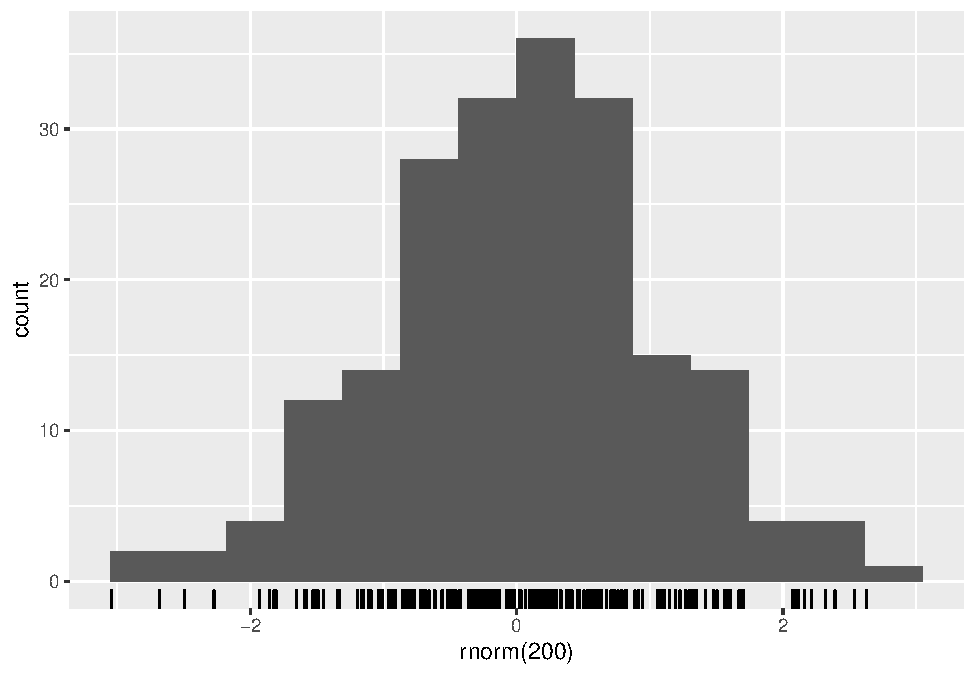
\includegraphics{bookdown-demo_files/figure-latex/unnamed-chunk-1-1.pdf}

\begin{Shaded}
\begin{Highlighting}[]
\CommentTok{# Equivalent to typing in the help menu }
\NormalTok{?mean }

\CommentTok{# Example in the help menu for the mean}
\NormalTok{x <-}\StringTok{ }\KeywordTok{c}\NormalTok{(}\DecValTok{0}\OperatorTok{:}\DecValTok{10}\NormalTok{, }\DecValTok{50}\NormalTok{) }
\KeywordTok{length}\NormalTok{(x)}
\end{Highlighting}
\end{Shaded}

\begin{verbatim}
## [1] 12
\end{verbatim}

\begin{Shaded}
\begin{Highlighting}[]
\NormalTok{xm <-}\StringTok{ }\KeywordTok{mean}\NormalTok{(x) }


\NormalTok{austa }\CommentTok{# what happens here? }
\end{Highlighting}
\end{Shaded}

\begin{verbatim}
## Time Series:
## Start = 1980 
## End = 2015 
## Frequency = 1 
##  [1] 0.8298943 0.8595109 0.8766892 0.8667072 0.9320520 1.0482636 1.3111932
##  [8] 1.6375623 2.0641074 1.9126828 2.0354457 2.1772113 2.3896834 2.7505921
## [15] 3.0906664 3.4266403 3.8306491 3.9719086 3.8316004 4.1431010 4.5665510
## [22] 4.4754100 4.4627960 4.3848290 4.7968610 5.0150490 5.0634350 5.1454890
## [29] 5.0994360 5.0881660 5.3537020 5.3433270 5.5891620 5.9048840 6.3571830
## [36] 6.8589530
\end{verbatim}

\begin{Shaded}
\begin{Highlighting}[]
\CommentTok{# Ignore the error message and keep going}



\CommentTok{# Lets look at some data sets from fpp}
\NormalTok{austa  }\CommentTok{#International vistors to Australia}
\end{Highlighting}
\end{Shaded}

\begin{verbatim}
## Time Series:
## Start = 1980 
## End = 2015 
## Frequency = 1 
##  [1] 0.8298943 0.8595109 0.8766892 0.8667072 0.9320520 1.0482636 1.3111932
##  [8] 1.6375623 2.0641074 1.9126828 2.0354457 2.1772113 2.3896834 2.7505921
## [15] 3.0906664 3.4266403 3.8306491 3.9719086 3.8316004 4.1431010 4.5665510
## [22] 4.4754100 4.4627960 4.3848290 4.7968610 5.0150490 5.0634350 5.1454890
## [29] 5.0994360 5.0881660 5.3537020 5.3433270 5.5891620 5.9048840 6.3571830
## [36] 6.8589530
\end{verbatim}

\begin{Shaded}
\begin{Highlighting}[]
\KeywordTok{autoplot}\NormalTok{(austa)}
\end{Highlighting}
\end{Shaded}

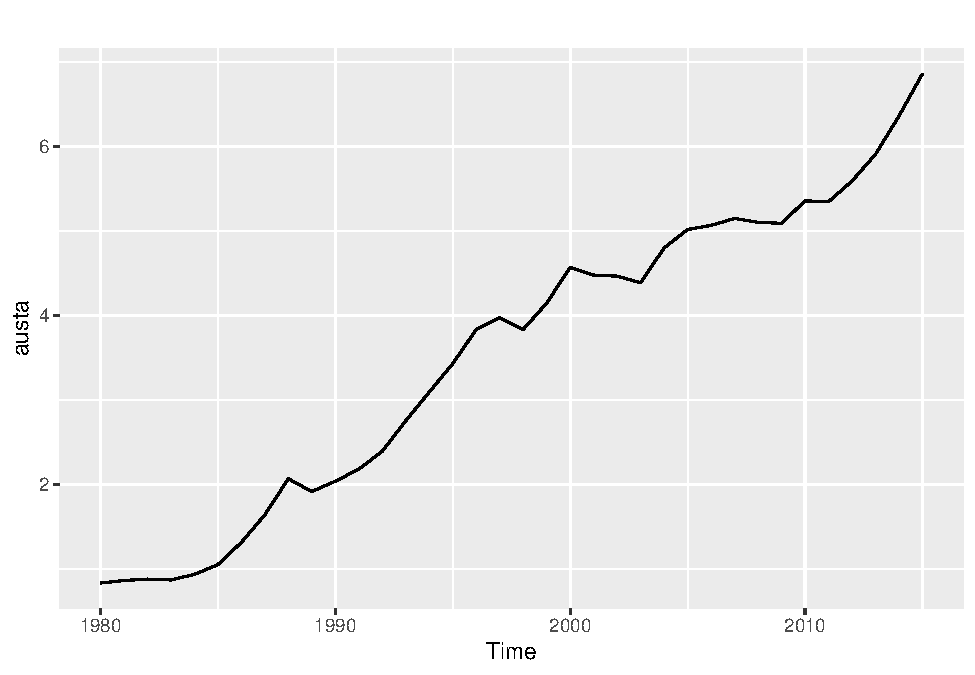
\includegraphics{bookdown-demo_files/figure-latex/unnamed-chunk-1-2.pdf}

\begin{Shaded}
\begin{Highlighting}[]
\CommentTok{# Summary command: prints an appropriate summary of what you asked from}
\KeywordTok{summary}\NormalTok{(austa)}
\end{Highlighting}
\end{Shaded}

\begin{verbatim}
##    Min. 1st Qu.  Median    Mean 3rd Qu.    Max. 
##  0.8299  2.0048  3.9018  3.5414  5.0696  6.8590
\end{verbatim}

\begin{Shaded}
\begin{Highlighting}[]
\CommentTok{# Some monthly data}
\NormalTok{a10 }\CommentTok{# Monthly anti-diabetic drug sales in Australia from 1992 to 2008}
\end{Highlighting}
\end{Shaded}

\begin{verbatim}
##            Jan       Feb       Mar       Apr       May       Jun       Jul
## 1991                                                              3.526591
## 1992  5.088335  2.814520  2.985811  3.204780  3.127578  3.270523  3.737851
## 1993  6.192068  3.450857  3.772307  3.734303  3.905399  4.049687  4.315566
## 1994  6.731473  3.841278  4.394076  4.075341  4.540645  4.645615  4.752607
## 1995  6.749484  4.216067  4.949349  4.823045  5.194754  5.170787  5.256742
## 1996  8.329452  5.069796  5.262557  5.597126  6.110296  5.689161  6.486849
## 1997  8.524471  5.277918  5.714303  6.214529  6.411929  6.667716  7.050831
## 1998  8.798513  5.918261  6.534493  6.675736  7.064201  7.383381  7.813496
## 1999 10.391416  6.421535  8.062619  7.297739  7.936916  8.165323  8.717420
## 2000 12.511462  7.457199  8.591191  8.474000  9.386803  9.560399 10.834295
## 2001 14.497581  8.049275 10.312891  9.753358 10.850382  9.961719 11.443601
## 2002 16.300269  9.053485 10.002449 10.788750 12.106705 10.954101 12.844566
## 2003 16.828350  9.800215 10.816994 10.654223 12.512323 12.161210 12.998046
## 2004 18.003768 11.938030 12.997900 12.882645 13.943447 13.989472 15.339097
## 2005 20.778723 12.154552 13.402392 14.459239 14.795102 15.705248 15.829550
## 2006 23.486694 12.536987 15.467018 14.233539 17.783058 16.291602 16.980282
## 2007 28.038383 16.763869 19.792754 16.427305 21.000742 20.681002 21.834890
## 2008 29.665356 21.654285 18.264945 23.107677 22.912510 19.431740          
##            Aug       Sep       Oct       Nov       Dec
## 1991  3.180891  3.252221  3.611003  3.565869  4.306371
## 1992  3.558776  3.777202  3.924490  4.386531  5.810549
## 1993  4.562185  4.608662  4.667851  5.093841  7.179962
## 1994  5.350605  5.204455  5.301651  5.773742  6.204593
## 1995  5.855277  5.490729  6.115293  6.088473  7.416598
## 1996  6.300569  6.467476  6.828629  6.649078  8.606937
## 1997  6.704919  7.250988  7.819733  7.398101 10.096233
## 1998  7.431892  8.275117  8.260441  8.596156 10.558939
## 1999  9.070964  9.177113  9.251887  9.933136 11.532974
## 2000 10.643751  9.908162 11.710041 11.340151 12.079132
## 2001 11.659239 10.647060 12.652134 13.674466 12.965735
## 2002 12.196500 12.854748 13.542004 13.287640 15.134918
## 2003 12.517276 13.268658 14.733622 13.669382 16.503966
## 2004 15.370764 16.142005 16.685754 17.636728 18.869325
## 2005 17.554701 18.100864 17.496668 19.347265 20.031291
## 2006 18.612189 16.623343 21.430241 23.575517 23.334206
## 2007 23.930204 22.930357 23.263340 25.250030 25.806090
## 2008
\end{verbatim}

\begin{Shaded}
\begin{Highlighting}[]
\KeywordTok{autoplot}\NormalTok{(a10)}
\end{Highlighting}
\end{Shaded}

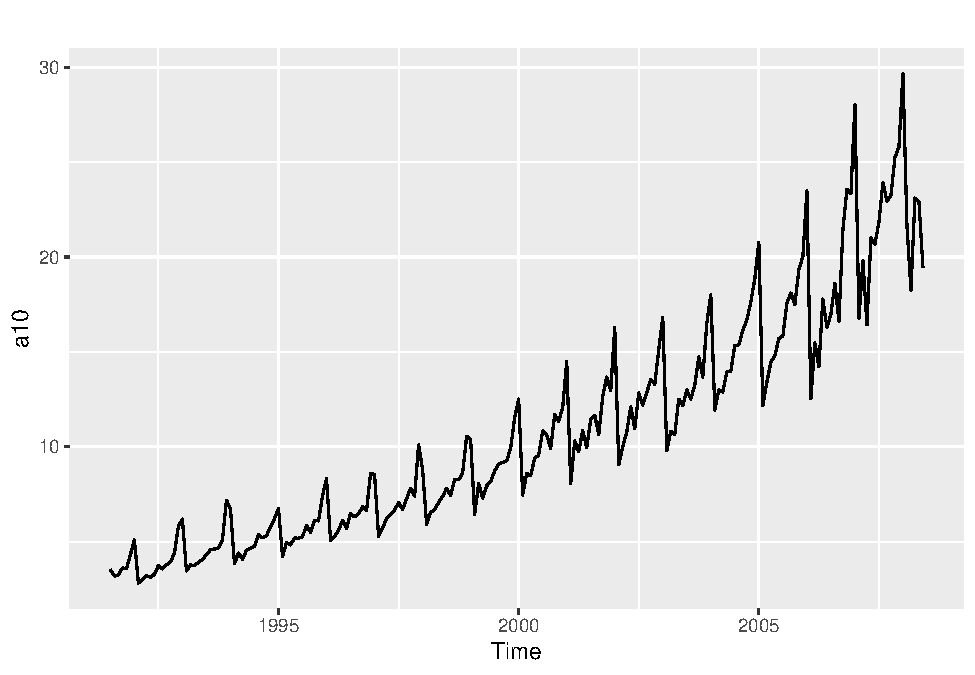
\includegraphics{bookdown-demo_files/figure-latex/unnamed-chunk-1-3.pdf}

\begin{Shaded}
\begin{Highlighting}[]
\KeywordTok{summary}\NormalTok{(a10)}
\end{Highlighting}
\end{Shaded}

\begin{verbatim}
##    Min. 1st Qu.  Median    Mean 3rd Qu.    Max. 
##   2.815   5.844   9.319  10.694  14.290  29.665
\end{verbatim}

\begin{Shaded}
\begin{Highlighting}[]
\CommentTok{# You will practice reading in your own data in the tutorials this week}
\CommentTok{# and next week. This will set you up well for the assignment}

\CommentTok{# This creates a vector y of observations}
\NormalTok{y=}\KeywordTok{c}\NormalTok{(}\DecValTok{1}\NormalTok{,}\DecValTok{2}\NormalTok{,}\DecValTok{3}\NormalTok{,}\DecValTok{4}\NormalTok{,}\DecValTok{5}\NormalTok{,}\DecValTok{6}\NormalTok{)}
\KeywordTok{mean}\NormalTok{(y)}
\end{Highlighting}
\end{Shaded}

\begin{verbatim}
## [1] 3.5
\end{verbatim}

\begin{Shaded}
\begin{Highlighting}[]
\CommentTok{# Write your own function }

\NormalTok{average<-}\ControlFlowTok{function}\NormalTok{(x)}
\NormalTok{\{}
  \KeywordTok{return}\NormalTok{(}\KeywordTok{sum}\NormalTok{(x)}\OperatorTok{/}\KeywordTok{length}\NormalTok{(x))}
\NormalTok{\}}

\NormalTok{ybar<-}\KeywordTok{average}\NormalTok{(y)}
\end{Highlighting}
\end{Shaded}

\hypertarget{lesson-2-time-series-graphic}{%
\section{Lesson 2: Time series graphic}\label{lesson-2-time-series-graphic}}

\begin{Shaded}
\begin{Highlighting}[]
\KeywordTok{library}\NormalTok{(fpp2)}

\CommentTok{# ts objects}
  
\NormalTok{x <-}\StringTok{ }\KeywordTok{c}\NormalTok{(}\DecValTok{123}\NormalTok{,}\DecValTok{39}\NormalTok{,}\DecValTok{78}\NormalTok{,}\DecValTok{52}\NormalTok{,}\DecValTok{110}\NormalTok{) }\CommentTok{# This is now just a column of numbers}
\NormalTok{x}
\end{Highlighting}
\end{Shaded}

\begin{verbatim}
## [1] 123  39  78  52 110
\end{verbatim}

\begin{Shaded}
\begin{Highlighting}[]
\KeywordTok{plot}\NormalTok{(x)}
\end{Highlighting}
\end{Shaded}

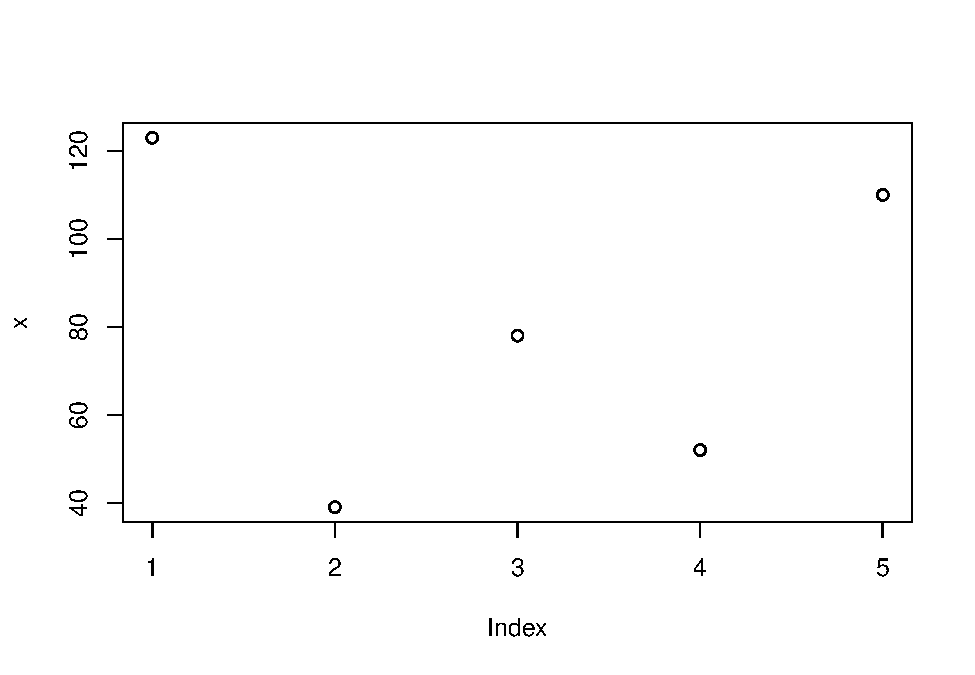
\includegraphics{bookdown-demo_files/figure-latex/unnamed-chunk-2-1.pdf}

\begin{Shaded}
\begin{Highlighting}[]
\NormalTok{  y <-}\StringTok{ }\KeywordTok{ts}\NormalTok{(}\KeywordTok{c}\NormalTok{(}\DecValTok{123}\NormalTok{,}\DecValTok{39}\NormalTok{,}\DecValTok{78}\NormalTok{,}\DecValTok{52}\NormalTok{,}\DecValTok{110}\NormalTok{), }\DataTypeTok{start=}\DecValTok{2012}\NormalTok{)}
\NormalTok{  y}
\end{Highlighting}
\end{Shaded}

\begin{verbatim}
## Time Series:
## Start = 2012 
## End = 2016 
## Frequency = 1 
## [1] 123  39  78  52 110
\end{verbatim}

\begin{Shaded}
\begin{Highlighting}[]
\KeywordTok{plot}\NormalTok{(y)}
\end{Highlighting}
\end{Shaded}

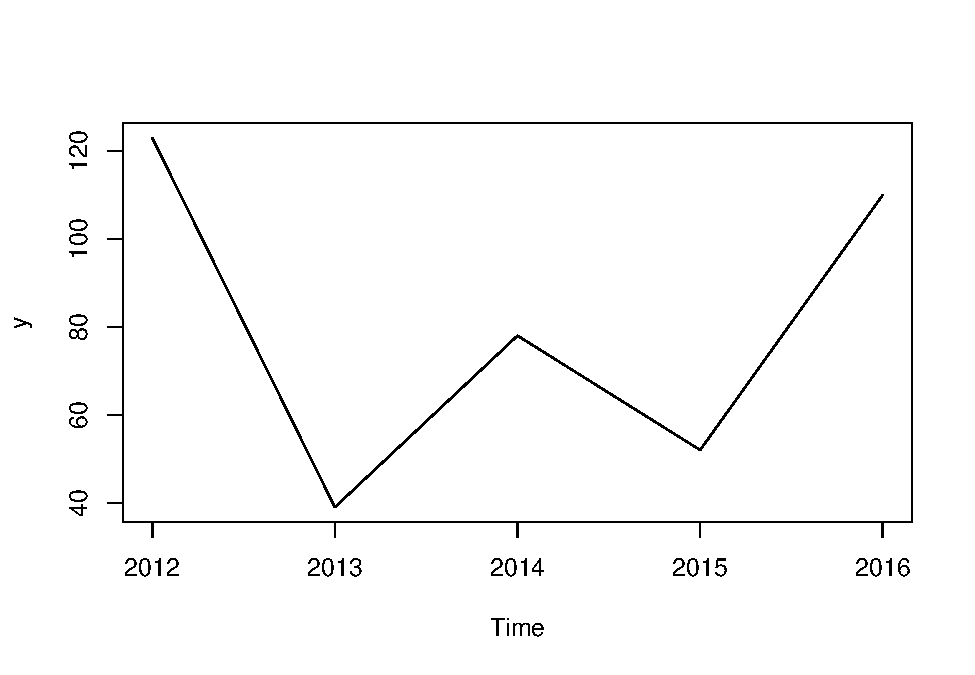
\includegraphics{bookdown-demo_files/figure-latex/unnamed-chunk-2-2.pdf}

\begin{Shaded}
\begin{Highlighting}[]
\NormalTok{  z <-}\StringTok{ }\KeywordTok{ts}\NormalTok{(x, }\DataTypeTok{frequency=}\DecValTok{12}\NormalTok{, }\DataTypeTok{start=}\KeywordTok{c}\NormalTok{(}\DecValTok{2003}\NormalTok{,}\DecValTok{1}\NormalTok{))}
\NormalTok{  z}
\end{Highlighting}
\end{Shaded}

\begin{verbatim}
##      Jan Feb Mar Apr May
## 2003 123  39  78  52 110
\end{verbatim}

\begin{Shaded}
\begin{Highlighting}[]
  \CommentTok{# For higher frequency data use the frequency argument }
  \CommentTok{#  setwd("C:/George/Teaching/ETF3231/2018/RinLectures")}
\NormalTok{x <-}\StringTok{ }\KeywordTok{scan}\NormalTok{(here}\OperatorTok{::}\KeywordTok{here}\NormalTok{(}\StringTok{"data"}\NormalTok{,}\StringTok{"gdp.dat"}\NormalTok{))}
  
\NormalTok{ausgdp <-}\StringTok{ }\KeywordTok{ts}\NormalTok{(x,}\DataTypeTok{frequency=}\DecValTok{4}\NormalTok{,}
             \DataTypeTok{start=}\FloatTok{1971.5}\NormalTok{) }\CommentTok{# Data starts in Q3}
  \KeywordTok{plot}\NormalTok{(ausgdp) }\CommentTok{# part of base graphics}
\end{Highlighting}
\end{Shaded}

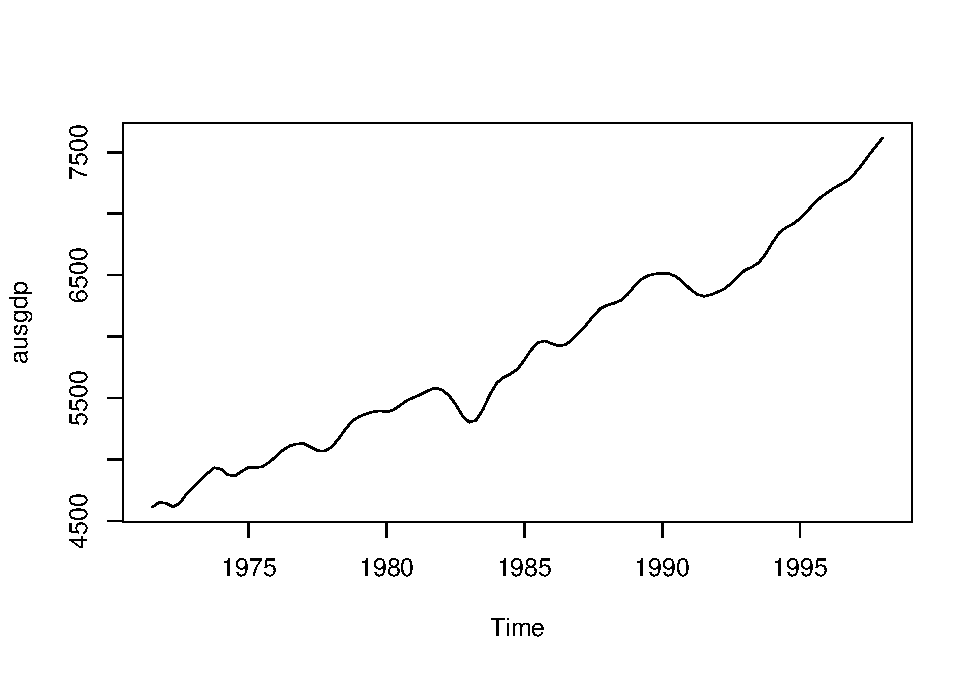
\includegraphics{bookdown-demo_files/figure-latex/unnamed-chunk-2-3.pdf}

\begin{Shaded}
\begin{Highlighting}[]
  \KeywordTok{autoplot}\NormalTok{(ausgdp)  }\CommentTok{# part of forecast and interaction with ggplot2}
\end{Highlighting}
\end{Shaded}

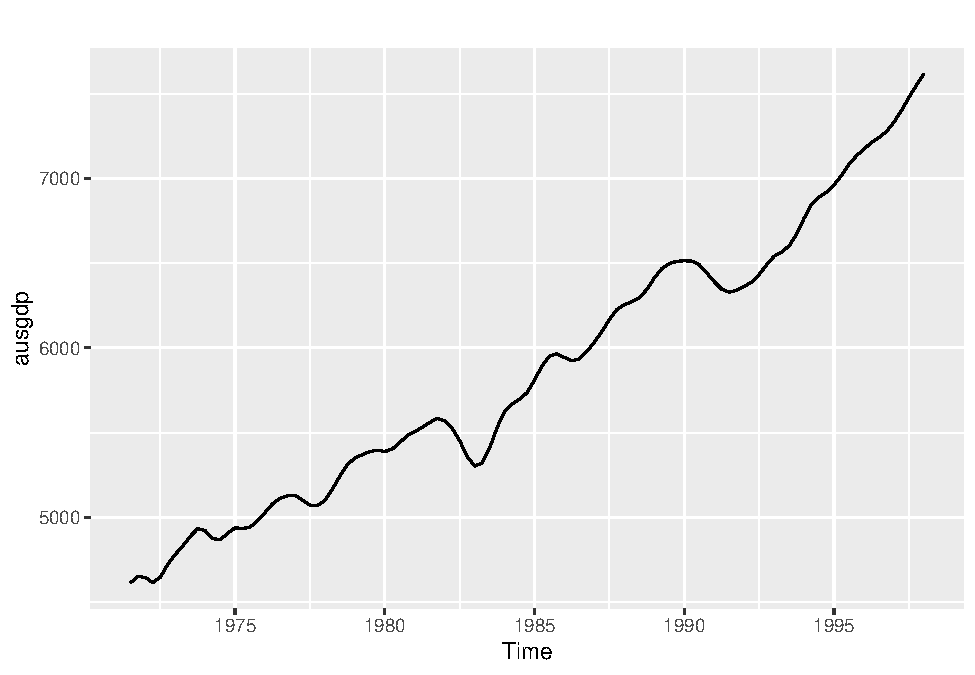
\includegraphics{bookdown-demo_files/figure-latex/unnamed-chunk-2-4.pdf}

\begin{Shaded}
\begin{Highlighting}[]
                    \CommentTok{# better plots only for ts objects}

\NormalTok{z=}\KeywordTok{rnorm}\NormalTok{(}\DecValTok{120}\NormalTok{)}
\CommentTok{#autoplot(z) }
\KeywordTok{plot}\NormalTok{(z)}
\end{Highlighting}
\end{Shaded}

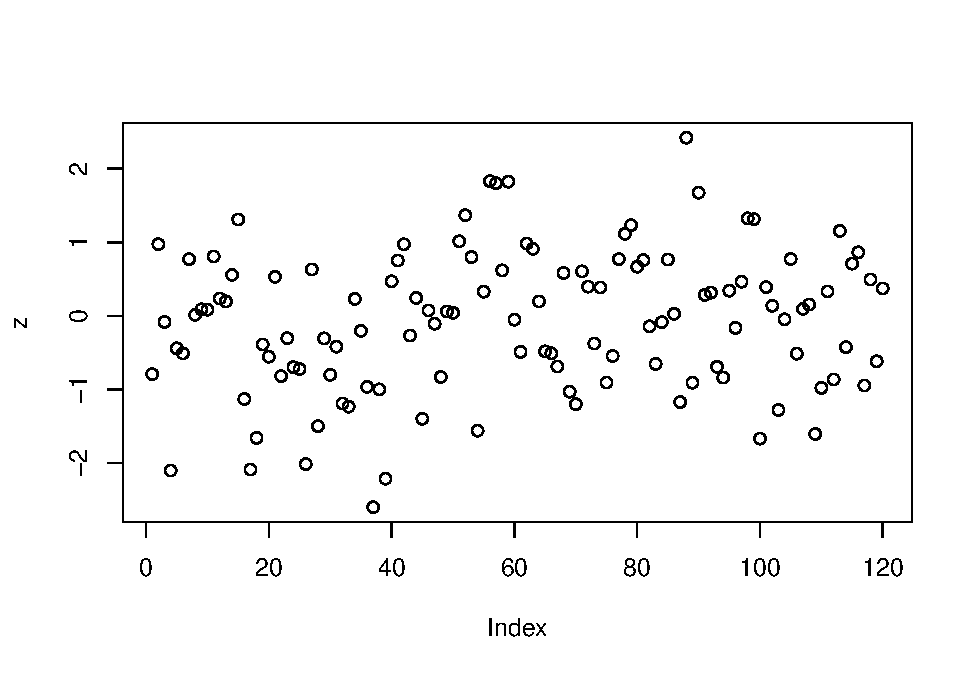
\includegraphics{bookdown-demo_files/figure-latex/unnamed-chunk-2-5.pdf}

\begin{Shaded}
\begin{Highlighting}[]
\NormalTok{  y <-}\StringTok{ }\KeywordTok{ts}\NormalTok{(z, }\DataTypeTok{start=}\DecValTok{2003}\NormalTok{, }\DataTypeTok{frequency=}\DecValTok{12}\NormalTok{)}
  \KeywordTok{attributes}\NormalTok{(y)}
\end{Highlighting}
\end{Shaded}

\begin{verbatim}
## $tsp
## [1] 2003.000 2012.917   12.000
## 
## $class
## [1] "ts"
\end{verbatim}

\begin{Shaded}
\begin{Highlighting}[]
  \KeywordTok{autoplot}\NormalTok{(y)}
\end{Highlighting}
\end{Shaded}

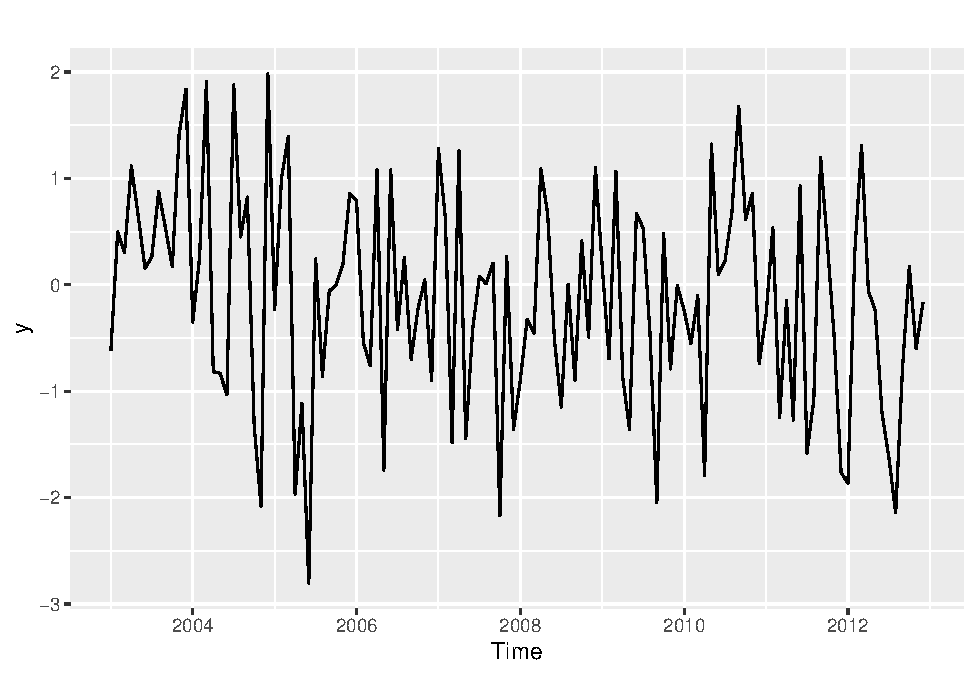
\includegraphics{bookdown-demo_files/figure-latex/unnamed-chunk-2-6.pdf}

\begin{Shaded}
\begin{Highlighting}[]
  \CommentTok{# Some ready ts}
\NormalTok{  elecsales}
\end{Highlighting}
\end{Shaded}

\begin{verbatim}
## Time Series:
## Start = 1989 
## End = 2008 
## Frequency = 1 
##  [1] 2354.34 2379.71 2318.52 2468.99 2386.09 2569.47 2575.72 2762.72 2844.50
## [10] 3000.70 3108.10 3357.50 3075.70 3180.60 3221.60 3176.20 3430.60 3527.48
## [19] 3637.89 3655.00
\end{verbatim}

\begin{Shaded}
\begin{Highlighting}[]
\NormalTok{  ?elecsales}
  \CommentTok{# Everyone to plot}
  \CommentTok{# Also ask them to use the help command - you will need to do }
  \CommentTok{# this a lot}
  
  \CommentTok{# ? is shorthand for help()}
  
  \CommentTok{# Ask everyone to type melsyd to see what they get}
  
\NormalTok{  melsyd }\CommentTok{# let's have a look}
\end{Highlighting}
\end{Shaded}

\begin{verbatim}
## Time Series:
## Start = c(1987, 26) 
## End = c(1992, 48) 
## Frequency = 52 
##          First.Class Business.Class Economy.Class
## 1987.481       1.912             NA        20.167
## 1987.500       1.848             NA        20.161
## 1987.519       1.856             NA        19.993
## 1987.538       2.142             NA        20.986
## 1987.558       2.118             NA        20.497
## 1987.577       2.048             NA        20.770
## 1987.596       2.111             NA        21.111
## 1987.615       2.199             NA        20.675
## 1987.635       2.231             NA        22.092
## 1987.654       2.081             NA        20.772
## 1987.673       2.213             NA        21.642
## 1987.692       2.131             NA        21.911
## 1987.712          NA             NA            NA
## 1987.731       2.131             NA        23.777
## 1987.750       2.034             NA        22.658
## 1987.769       2.190             NA        23.515
## 1987.788       2.262             NA        21.384
## 1987.808       2.579             NA        24.344
## 1987.827       2.367             NA        21.137
## 1987.846       2.432             NA        23.069
## 1987.865       2.640             NA        23.664
## 1987.885       2.614             NA        23.219
## 1987.904       2.569             NA        23.192
## 1987.923       2.523             NA        23.475
## 1987.942       2.260             NA        22.377
## 1987.962       1.117             NA        16.606
## 1987.981       0.590             NA        13.987
## 1988.000       0.966             NA        16.251
## 1988.019       1.235             NA        18.439
## 1988.038       2.001             NA        20.262
## 1988.058       1.696             NA        19.535
## 1988.077       2.089             NA        22.467
## 1988.096       2.716             NA        24.559
## 1988.115       2.483             NA        24.591
## 1988.135       2.461             NA        24.511
## 1988.154       2.533             NA        24.524
## 1988.173       2.273             NA        23.119
## 1988.192       2.273             NA        23.106
## 1988.212       2.370             NA        23.292
## 1988.231       1.782             NA        21.566
## 1988.250       1.385             NA        18.565
## 1988.269       2.322             NA        24.361
## 1988.288       2.340             NA        22.983
## 1988.308       2.203             NA        21.062
## 1988.327       2.300             NA        21.766
## 1988.346       2.125             NA        22.285
## 1988.365       2.345             NA        22.867
## 1988.385       2.224             NA        23.276
## 1988.404       1.952             NA        20.924
## 1988.423       2.212             NA        21.716
## 1988.442       2.028             NA        20.908
## 1988.462       1.906             NA        21.410
## 1988.481       1.834             NA        21.361
## 1988.500       1.797             NA        22.412
## 1988.519       1.869             NA        21.290
## 1988.538       1.886             NA        22.247
## 1988.558       2.131             NA        22.445
## 1988.577       2.021             NA        21.260
## 1988.596       2.199             NA        22.771
## 1988.615       2.140             NA        23.723
## 1988.635       2.190             NA        23.757
## 1988.654       1.917             NA        23.482
## 1988.673       2.096             NA        23.653
## 1988.692       2.254             NA        26.054
## 1988.712       2.251             NA        25.695
## 1988.731       2.072             NA        26.720
## 1988.750       0.993             NA        15.033
## 1988.769       1.675             NA        22.340
## 1988.788       1.463             NA        19.297
## 1988.808       2.256             NA        23.761
## 1988.827       2.216             NA        22.150
## 1988.846       2.218             NA        22.236
## 1988.865       2.568             NA        23.157
## 1988.885       2.483             NA        24.387
## 1988.904       2.545             NA        23.844
## 1988.923       2.599             NA        23.681
## 1988.942       2.483             NA        24.456
## 1988.962       1.793             NA        19.899
## 1988.981       0.516             NA        13.662
## 1989.000       0.873             NA        15.698
## 1989.019       1.195             NA        18.189
## 1989.038       1.525             NA        19.448
## 1989.058       1.906             NA        20.891
## 1989.077       2.246             NA        22.284
## 1989.096       2.247             NA        23.247
## 1989.115       2.316             NA        24.440
## 1989.135       2.276             NA        22.519
## 1989.154       2.403             NA        22.818
## 1989.173       2.432             NA        23.472
## 1989.192       2.490             NA        24.117
## 1989.212       2.013             NA        24.435
## 1989.231       1.508             NA        20.589
## 1989.250       2.251             NA        23.427
## 1989.269       2.079             NA        20.923
## 1989.288       2.210             NA        22.959
## 1989.308       1.960             NA        19.152
## 1989.327       2.251             NA        22.011
## 1989.346       2.013             NA        20.228
## 1989.365       2.252             NA        21.332
## 1989.385       2.067             NA        20.500
## 1989.404       1.831             NA        19.090
## 1989.423       2.069             NA        21.692
## 1989.442       1.953             NA        20.157
## 1989.462       2.199             NA        22.231
## 1989.481       1.771             NA        20.914
## 1989.500       1.696             NA        21.454
## 1989.519       1.788             NA        21.345
## 1989.538       1.636          1.524        19.260
## 1989.558       1.741          2.212        18.781
## 1989.577       1.597          1.777        17.445
## 1989.596       1.943          2.552        19.628
## 1989.615       1.660          1.889        17.692
## 1989.635       0.616          0.851         7.046
## 1989.654       0.000          0.000         0.000
## 1989.673       0.000          0.000         0.000
## 1989.692       0.000          0.000         0.000
## 1989.712       0.000          0.000         0.000
## 1989.731       0.000          0.000         0.000
## 1989.750       0.000          0.000         0.000
## 1989.769       0.000          0.000         0.000
## 1989.788       0.053          0.618        11.569
## 1989.808       0.040          0.565        11.973
## 1989.827       0.354          0.414        11.123
## 1989.846       0.505          0.543        11.479
## 1989.865       0.711          0.712        16.969
## 1989.885       0.723          0.652        15.997
## 1989.904       0.796          0.709        16.555
## 1989.923       0.856          0.793        17.959
## 1989.942       0.845          0.838        18.868
## 1989.962       0.807          0.763        15.400
## 1989.981       0.276          0.266        10.544
## 1990.000       0.339          0.362        12.755
## 1990.019       0.581          0.665        19.020
## 1990.038       0.894          0.957        20.077
## 1990.058       0.936          1.145        22.124
## 1990.077       1.111          1.312        19.920
## 1990.096       1.446          1.689        17.215
## 1990.115       1.517          1.762        17.662
## 1990.135       1.513          2.160        19.828
## 1990.154       1.508          1.877        18.754
## 1990.173       1.636          2.048        20.390
## 1990.192       1.380          1.824        18.383
## 1990.212       1.453          1.986        19.377
## 1990.231       1.459          2.032        20.133
## 1990.250       1.538          1.956        19.210
## 1990.269       1.327          1.503        20.736
## 1990.288       1.027          1.256        18.821
## 1990.308       1.365          1.752        20.952
## 1990.327       1.475          1.878        20.565
## 1990.346       1.365          1.945        20.311
## 1990.365       1.351          1.735        17.859
## 1990.385       1.231          1.825        19.385
## 1990.404       1.447          1.715        17.962
## 1990.423       1.408          1.594        19.569
## 1990.442       1.089          1.377        17.894
## 1990.462       1.357          1.686        18.114
## 1990.481       1.287          1.560        19.170
## 1990.500       1.087          1.692        18.713
## 1990.519       1.017          1.597        20.520
## 1990.538       1.090          1.729        20.345
## 1990.558       1.343          1.733        20.015
## 1990.577       1.164          1.813        18.027
## 1990.596       1.169          1.725        19.697
## 1990.615       1.465          1.909        19.897
## 1990.635       1.242          1.765        19.213
## 1990.654       1.220          1.781        19.773
## 1990.673       1.231          1.717        20.128
## 1990.692       1.266          1.884        21.181
## 1990.712       1.337          1.881        21.933
## 1990.731       1.079          1.433        20.049
## 1990.750       1.223          1.534        23.358
## 1990.769       1.351          1.926        21.120
## 1990.788       1.269          1.870        21.970
## 1990.808       1.382          1.942        21.411
## 1990.827       1.435          2.222        22.569
## 1990.846       1.371          1.909        20.849
## 1990.865       1.341          2.089        20.658
## 1990.885       1.399          2.026        21.192
## 1990.904       1.440          2.009        21.502
## 1990.923       1.236          2.034        22.152
## 1990.942       1.441          2.085        21.904
## 1990.962       0.988          1.330        20.634
## 1990.981       0.300          0.318        15.535
## 1991.000       0.401          0.522        16.690
## 1991.019       0.529          0.824        19.150
## 1991.038       0.786          1.113        21.128
## 1991.058       1.086          1.285        21.136
## 1991.077       0.725          1.107        19.693
## 1991.096       1.127          1.591        21.576
## 1991.115       1.146          1.726        21.449
## 1991.135       1.086          1.758        22.298
## 1991.154       1.134          1.883        21.056
## 1991.173       1.020          2.089        19.014
## 1991.192       1.022          2.198        19.511
## 1991.212       1.224          2.449        20.162
## 1991.231       0.895          1.739        21.158
## 1991.250       0.658          1.480        19.059
## 1991.269       0.977          2.152        21.972
## 1991.288       0.916          2.258        22.877
## 1991.308       0.830          1.776        22.190
## 1991.327       0.990          2.355        22.533
## 1991.346       0.770          2.140        20.682
## 1991.365       0.801          1.988        21.788
## 1991.385       0.839          2.083        21.299
## 1991.404       0.835          2.115        20.663
## 1991.423       0.802          1.884        21.948
## 1991.442       0.763          1.797        21.009
## 1991.462       0.770          1.944        20.443
## 1991.481       0.838          2.001        21.418
## 1991.500       0.742          1.668        23.273
## 1991.519       0.793          1.527        25.763
## 1991.538       0.900          1.477        26.045
## 1991.558       0.960          1.949        23.831
## 1991.577       0.800          1.914        22.742
## 1991.596       0.807          1.632        22.962
## 1991.615       0.841          1.796        25.253
## 1991.635       0.880          1.696        25.239
## 1991.654       0.818          1.718        27.387
## 1991.673       0.817          1.442        26.824
## 1991.692       0.819          1.713        27.294
## 1991.712       0.998          1.796        28.935
## 1991.731       1.220          1.860        31.642
## 1991.750       0.966          1.554        32.468
## 1991.769       0.895          1.623        27.673
## 1991.788       0.978          1.641        28.890
## 1991.808       0.913          1.818        26.465
## 1991.827       0.947          1.969        28.296
## 1991.846       1.002          1.886        29.274
## 1991.865       1.081          2.030        30.686
## 1991.885       0.977          1.883        29.786
## 1991.904       1.027          1.871        31.155
## 1991.923       0.895          1.910        28.459
## 1991.942       0.900          1.921        27.195
## 1991.962       0.762          1.672        26.274
## 1991.981       0.329          0.386        25.204
## 1992.000       0.351          0.446        24.434
## 1992.019       0.419          0.819        27.323
## 1992.038       0.618          1.238        27.303
## 1992.058       0.845          1.761        30.334
## 1992.077       0.727          1.650        26.833
## 1992.096       1.200          2.031        25.811
## 1992.115       1.801          2.064        27.238
## 1992.135       1.727          2.418        28.788
## 1992.154       1.992          2.171        27.263
## 1992.173       1.865          2.362        27.217
## 1992.192       1.801          2.328        26.410
## 1992.212       1.661          2.336        26.118
## 1992.231       2.366         10.301        18.642
## 1992.250       2.003          9.964        16.518
## 1992.269       2.092         10.433        17.276
## 1992.288       1.703          8.281        21.662
## 1992.308       1.337          6.128        20.473
## 1992.327       1.985          9.709        18.336
## 1992.346       1.808          8.828        17.018
## 1992.365       1.839          8.078        18.111
## 1992.385       1.714          7.527        18.410
## 1992.404       1.730          7.486        20.541
## 1992.423       1.725          6.711        21.408
## 1992.442       1.456          5.930        21.545
## 1992.462       1.447          5.462        21.732
## 1992.481       1.357          3.710        26.173
## 1992.500       1.280          2.894        27.432
## 1992.519       1.363          3.008        28.362
## 1992.538       1.228          2.829        29.827
## 1992.558       1.411          3.252        29.870
## 1992.577       1.130          3.021        26.534
## 1992.596       1.153          2.667        26.434
## 1992.615       1.257          2.740        26.137
## 1992.635       1.259          2.807        27.365
## 1992.654       1.153          2.961        27.910
## 1992.673       1.202          2.570        26.311
## 1992.692       1.185          2.671        27.538
## 1992.712       1.247          2.809        29.445
## 1992.731       1.434          2.712        28.326
## 1992.750       1.450          2.606        30.203
## 1992.769       1.227          2.500        27.838
## 1992.788       1.245          2.898        27.760
## 1992.808       1.417          3.152        27.322
## 1992.827       1.458          3.053        28.837
## 1992.846       1.398          2.745        26.548
## 1992.865       1.423          3.156        27.279
## 1992.885       1.358          3.069        27.306
## 1992.904       1.488          3.379        28.299
\end{verbatim}

\begin{Shaded}
\begin{Highlighting}[]
  \KeywordTok{head}\NormalTok{(melsyd)}
\end{Highlighting}
\end{Shaded}

\begin{verbatim}
## Time Series:
## Start = c(1987, 26) 
## End = c(1987, 31) 
## Frequency = 52 
##          First.Class Business.Class Economy.Class
## 1987.481       1.912             NA        20.167
## 1987.500       1.848             NA        20.161
## 1987.519       1.856             NA        19.993
## 1987.538       2.142             NA        20.986
## 1987.558       2.118             NA        20.497
## 1987.577       2.048             NA        20.770
\end{verbatim}

\begin{Shaded}
\begin{Highlighting}[]
  \KeywordTok{tail}\NormalTok{(melsyd)}
\end{Highlighting}
\end{Shaded}

\begin{verbatim}
## Time Series:
## Start = c(1992, 43) 
## End = c(1992, 48) 
## Frequency = 52 
##          First.Class Business.Class Economy.Class
## 1992.808       1.417          3.152        27.322
## 1992.827       1.458          3.053        28.837
## 1992.846       1.398          2.745        26.548
## 1992.865       1.423          3.156        27.279
## 1992.885       1.358          3.069        27.306
## 1992.904       1.488          3.379        28.299
\end{verbatim}

\begin{Shaded}
\begin{Highlighting}[]
  \KeywordTok{autoplot}\NormalTok{(melsyd)}
\end{Highlighting}
\end{Shaded}

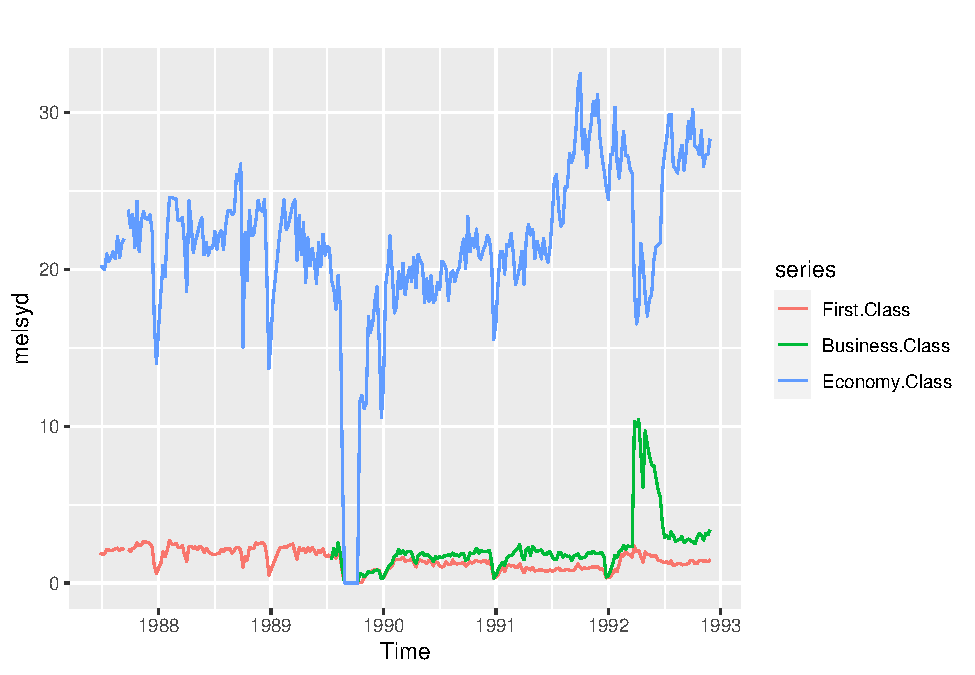
\includegraphics{bookdown-demo_files/figure-latex/unnamed-chunk-2-7.pdf}

\begin{Shaded}
\begin{Highlighting}[]
  \KeywordTok{autoplot}\NormalTok{(melsyd,}\DataTypeTok{facets =} \OtherTok{TRUE}\NormalTok{)}
\end{Highlighting}
\end{Shaded}

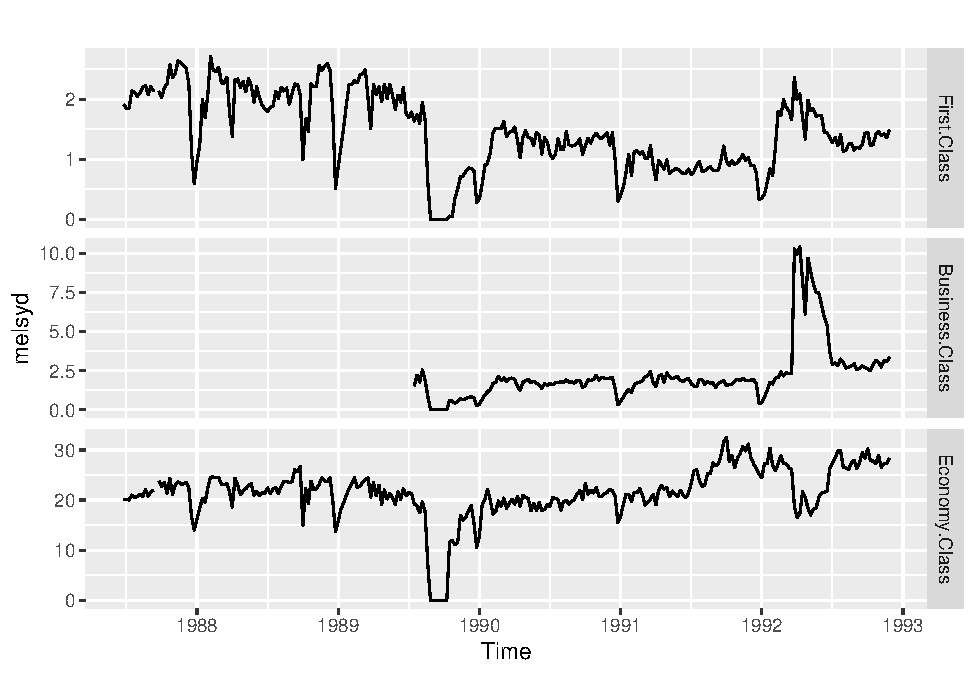
\includegraphics{bookdown-demo_files/figure-latex/unnamed-chunk-2-8.pdf}

\begin{Shaded}
\begin{Highlighting}[]
\CommentTok{# Back to slides}
  
  \CommentTok{# Time plot}
  \KeywordTok{autoplot}\NormalTok{(melsyd[,}\StringTok{"Economy.Class"}\NormalTok{])}
\end{Highlighting}
\end{Shaded}

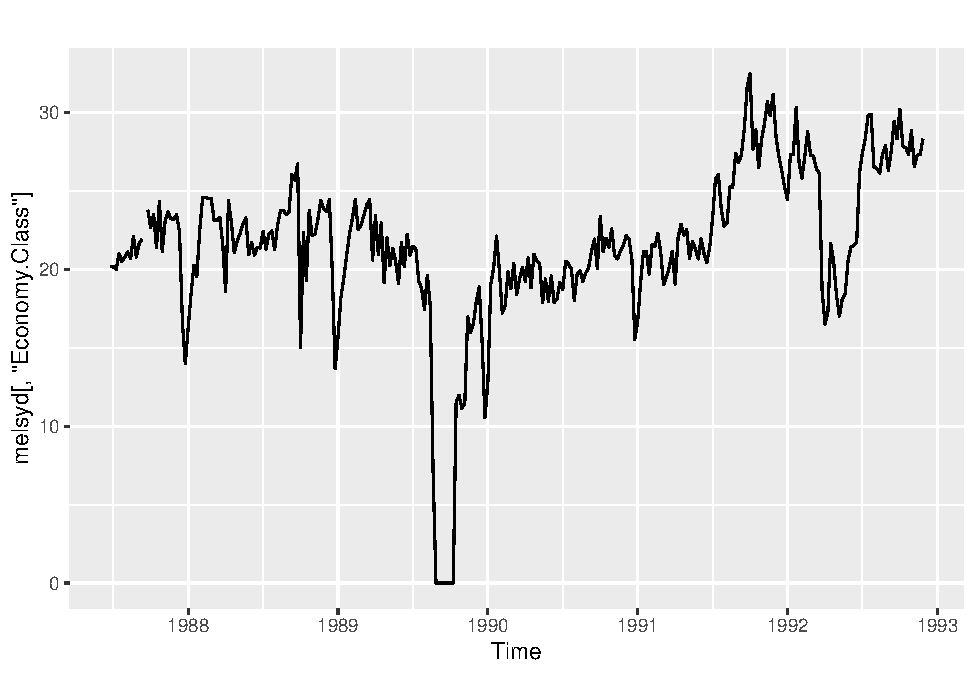
\includegraphics{bookdown-demo_files/figure-latex/unnamed-chunk-2-9.pdf}

\begin{Shaded}
\begin{Highlighting}[]
  \CommentTok{# Adding main title and }
  \CommentTok{# also add labels to the x and y axes}

  \KeywordTok{autoplot}\NormalTok{(a10) }\OperatorTok{+}\StringTok{ }\KeywordTok{ylab}\NormalTok{(}\StringTok{"$ million"}\NormalTok{) }\OperatorTok{+}\StringTok{ }\KeywordTok{xlab}\NormalTok{(}\StringTok{"Year"}\NormalTok{) }\OperatorTok{+}
\StringTok{    }\KeywordTok{ggtitle}\NormalTok{(}\StringTok{"Antidiabetic drug sales"}\NormalTok{)}
\end{Highlighting}
\end{Shaded}

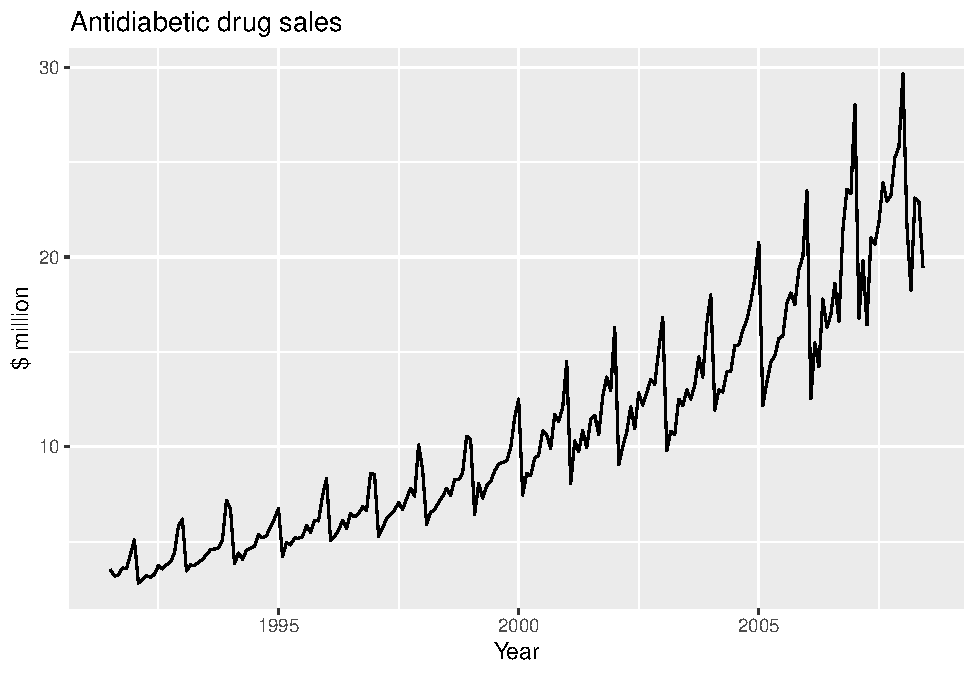
\includegraphics{bookdown-demo_files/figure-latex/unnamed-chunk-2-10.pdf}

\begin{Shaded}
\begin{Highlighting}[]
\NormalTok{  ?autoplot}
\end{Highlighting}
\end{Shaded}

\begin{verbatim}
## Help on topic 'autoplot' was found in the following packages:
## 
##   Package               Library
##   forecast              /Library/Frameworks/R.framework/Versions/4.0/Resources/library
##   ggplot2               /Library/Frameworks/R.framework/Versions/4.0/Resources/library
## 
## 
## Using the first match ...
\end{verbatim}

\begin{Shaded}
\begin{Highlighting}[]
\CommentTok{# Your turn}
  
\NormalTok{  ?dole}
  \KeywordTok{autoplot}\NormalTok{(dole)}
\end{Highlighting}
\end{Shaded}

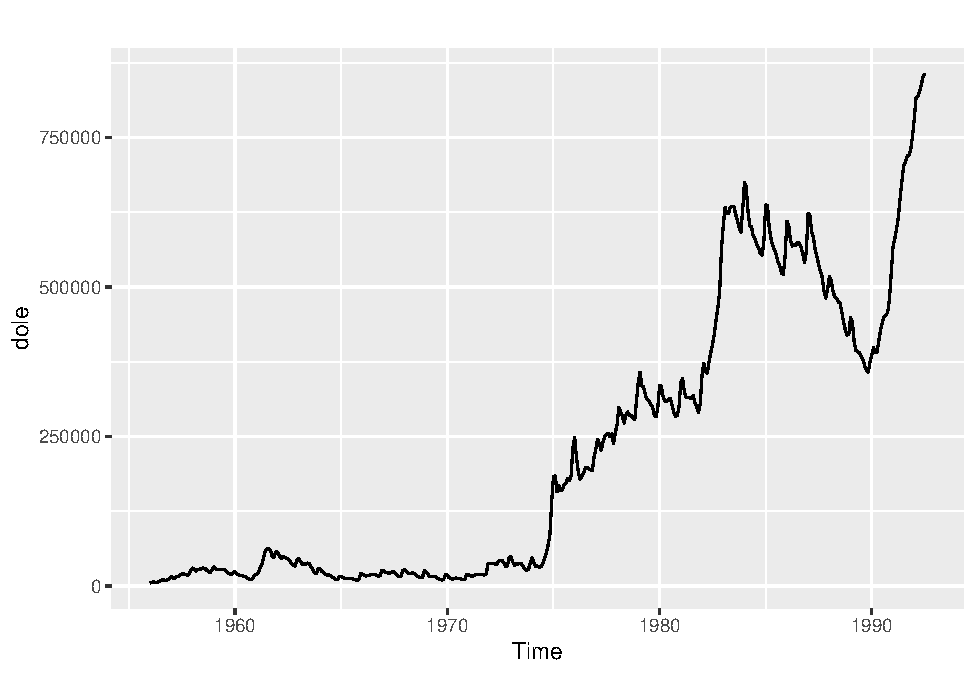
\includegraphics{bookdown-demo_files/figure-latex/unnamed-chunk-2-11.pdf}

\begin{Shaded}
\begin{Highlighting}[]
\NormalTok{  ?lynx}
\end{Highlighting}
\end{Shaded}

\begin{verbatim}
## Help on topic 'lynx' was found in the following packages:
## 
##   Package               Library
##   fma                   /Library/Frameworks/R.framework/Versions/4.0/Resources/library
##   datasets              /Library/Frameworks/R.framework/Versions/4.0/Resources/library
## 
## 
## Using the first match ...
\end{verbatim}

\begin{Shaded}
\begin{Highlighting}[]
  \KeywordTok{autoplot}\NormalTok{(lynx)}
\end{Highlighting}
\end{Shaded}

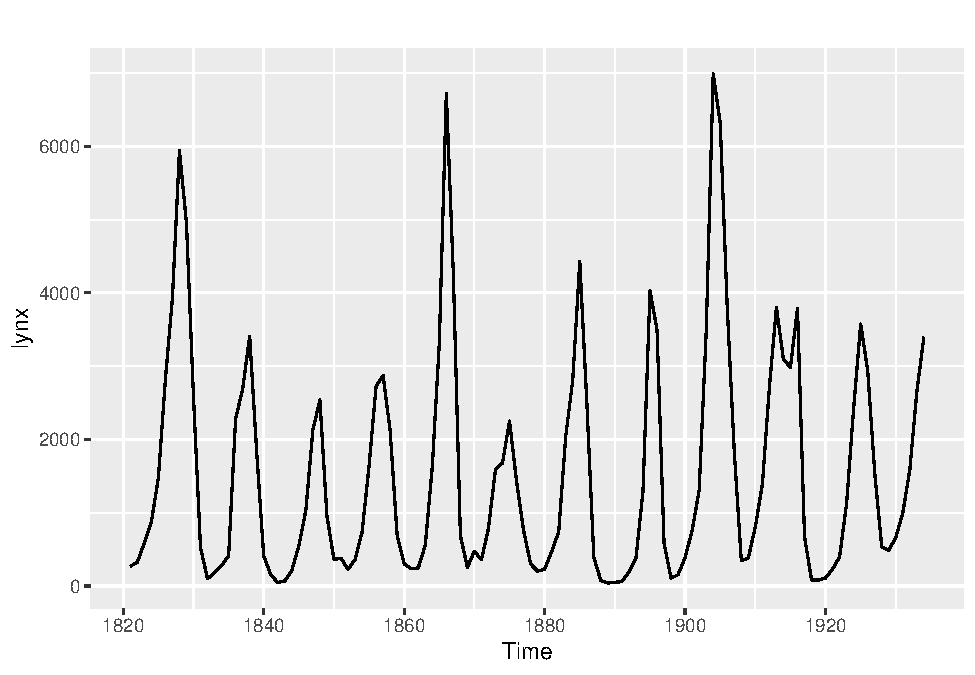
\includegraphics{bookdown-demo_files/figure-latex/unnamed-chunk-2-12.pdf}

\begin{Shaded}
\begin{Highlighting}[]
\NormalTok{  ?goog}
  
  \KeywordTok{autoplot}\NormalTok{(goog)}\OperatorTok{+}\StringTok{ }
\StringTok{    }\KeywordTok{xlab}\NormalTok{(}\StringTok{"Year"}\NormalTok{) }\OperatorTok{+}\StringTok{ }\KeywordTok{ylab}\NormalTok{(}\StringTok{"Price ($)"}\NormalTok{) }\OperatorTok{+}\StringTok{ }
\StringTok{    }\KeywordTok{ggtitle}\NormalTok{(}\StringTok{"Google closing stock price"}\NormalTok{)}
\end{Highlighting}
\end{Shaded}

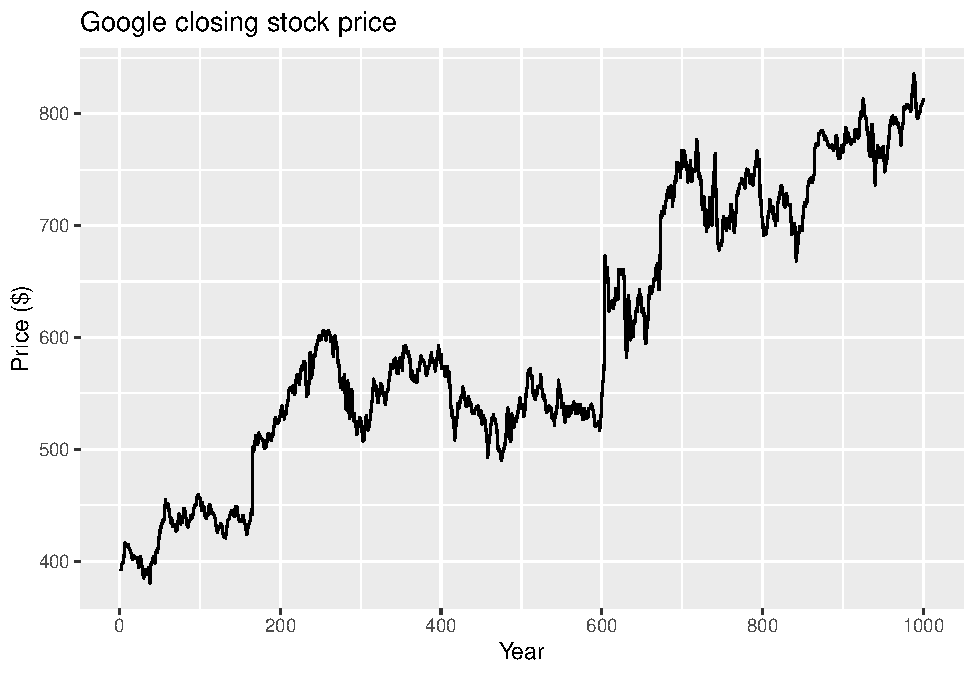
\includegraphics{bookdown-demo_files/figure-latex/unnamed-chunk-2-13.pdf}

\begin{Shaded}
\begin{Highlighting}[]
\CommentTok{# Back to slides}

  \CommentTok{# The elecdaily data}
\NormalTok{  ?elecdaily}
  \KeywordTok{head}\NormalTok{(elecdaily,}\DecValTok{15}\NormalTok{)}
\end{Highlighting}
\end{Shaded}

\begin{verbatim}
## Time Series:
## Start = c(1, 4) 
## End = c(3, 4) 
## Frequency = 7 
##            Demand WorkDay Temperature
## 1.428571 174.8963       0        26.0
## 1.571429 188.5909       1        23.0
## 1.714286 188.9169       1        22.2
## 1.857143 173.8142       0        20.3
## 2.000000 169.5152       0        26.1
## 2.142857 195.7288       1        19.6
## 2.285714 199.9029       1        20.0
## 2.428571 205.3375       1        27.4
## 2.571429 228.0782       1        32.4
## 2.714286 258.5984       1        34.0
## 2.857143 201.7970       0        22.4
## 3.000000 187.6298       0        22.5
## 3.142857 254.6636       1        30.0
## 3.285714 322.2323       1        42.4
## 3.428571 343.9934       1        41.5
\end{verbatim}

\begin{Shaded}
\begin{Highlighting}[]
  \KeywordTok{autoplot}\NormalTok{(elecdaily)}
\end{Highlighting}
\end{Shaded}

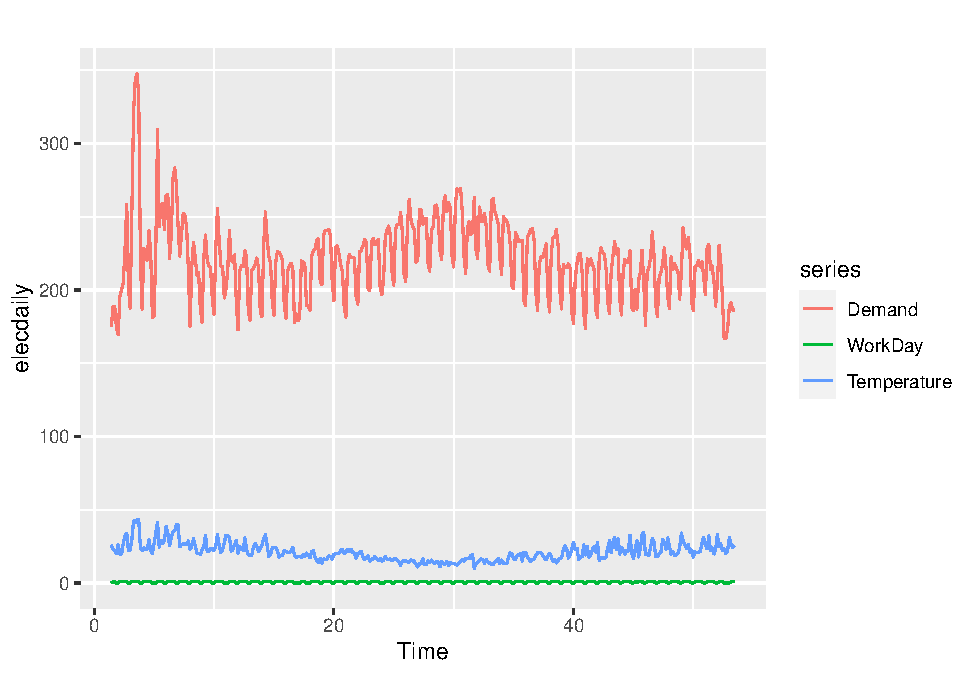
\includegraphics{bookdown-demo_files/figure-latex/unnamed-chunk-2-14.pdf}

\begin{Shaded}
\begin{Highlighting}[]
  \KeywordTok{autoplot}\NormalTok{(elecdaily[,}\DecValTok{3}\NormalTok{])}
\end{Highlighting}
\end{Shaded}

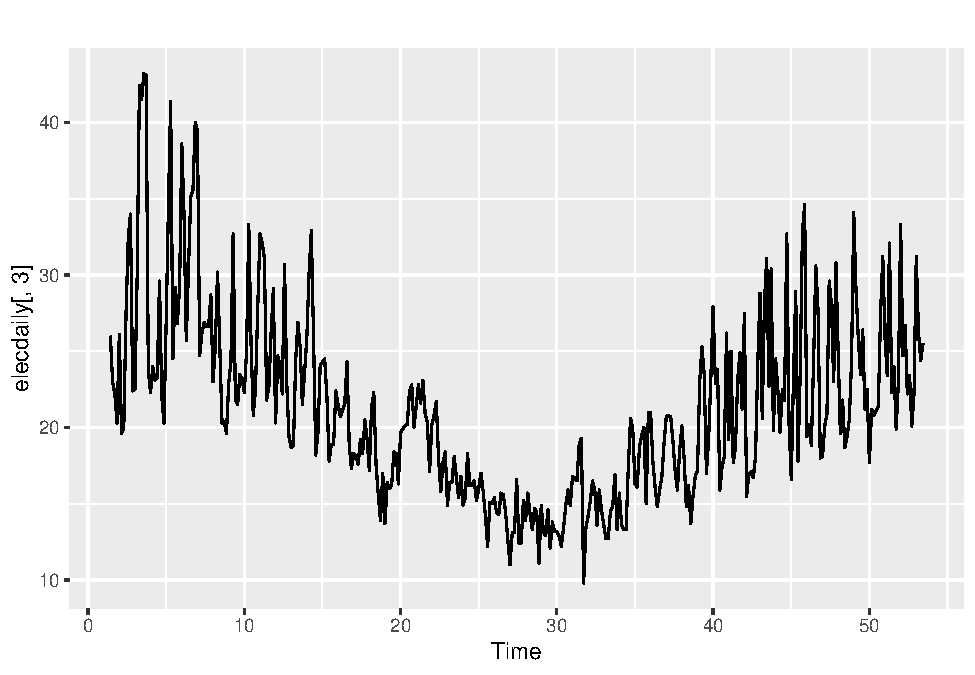
\includegraphics{bookdown-demo_files/figure-latex/unnamed-chunk-2-15.pdf}

\begin{Shaded}
\begin{Highlighting}[]
  \KeywordTok{time}\NormalTok{(elecdaily)}
\end{Highlighting}
\end{Shaded}

\begin{verbatim}
## Time Series:
## Start = c(1, 4) 
## End = c(53, 4) 
## Frequency = 7 
##   [1]  1.428571  1.571429  1.714286  1.857143  2.000000  2.142857  2.285714
##   [8]  2.428571  2.571429  2.714286  2.857143  3.000000  3.142857  3.285714
##  [15]  3.428571  3.571429  3.714286  3.857143  4.000000  4.142857  4.285714
##  [22]  4.428571  4.571429  4.714286  4.857143  5.000000  5.142857  5.285714
##  [29]  5.428571  5.571429  5.714286  5.857143  6.000000  6.142857  6.285714
##  [36]  6.428571  6.571429  6.714286  6.857143  7.000000  7.142857  7.285714
##  [43]  7.428571  7.571429  7.714286  7.857143  8.000000  8.142857  8.285714
##  [50]  8.428571  8.571429  8.714286  8.857143  9.000000  9.142857  9.285714
##  [57]  9.428571  9.571429  9.714286  9.857143 10.000000 10.142857 10.285714
##  [64] 10.428571 10.571429 10.714286 10.857143 11.000000 11.142857 11.285714
##  [71] 11.428571 11.571429 11.714286 11.857143 12.000000 12.142857 12.285714
##  [78] 12.428571 12.571429 12.714286 12.857143 13.000000 13.142857 13.285714
##  [85] 13.428571 13.571429 13.714286 13.857143 14.000000 14.142857 14.285714
##  [92] 14.428571 14.571429 14.714286 14.857143 15.000000 15.142857 15.285714
##  [99] 15.428571 15.571429 15.714286 15.857143 16.000000 16.142857 16.285714
## [106] 16.428571 16.571429 16.714286 16.857143 17.000000 17.142857 17.285714
## [113] 17.428571 17.571429 17.714286 17.857143 18.000000 18.142857 18.285714
## [120] 18.428571 18.571429 18.714286 18.857143 19.000000 19.142857 19.285714
## [127] 19.428571 19.571429 19.714286 19.857143 20.000000 20.142857 20.285714
## [134] 20.428571 20.571429 20.714286 20.857143 21.000000 21.142857 21.285714
## [141] 21.428571 21.571429 21.714286 21.857143 22.000000 22.142857 22.285714
## [148] 22.428571 22.571429 22.714286 22.857143 23.000000 23.142857 23.285714
## [155] 23.428571 23.571429 23.714286 23.857143 24.000000 24.142857 24.285714
## [162] 24.428571 24.571429 24.714286 24.857143 25.000000 25.142857 25.285714
## [169] 25.428571 25.571429 25.714286 25.857143 26.000000 26.142857 26.285714
## [176] 26.428571 26.571429 26.714286 26.857143 27.000000 27.142857 27.285714
## [183] 27.428571 27.571429 27.714286 27.857143 28.000000 28.142857 28.285714
## [190] 28.428571 28.571429 28.714286 28.857143 29.000000 29.142857 29.285714
## [197] 29.428571 29.571429 29.714286 29.857143 30.000000 30.142857 30.285714
## [204] 30.428571 30.571429 30.714286 30.857143 31.000000 31.142857 31.285714
## [211] 31.428571 31.571429 31.714286 31.857143 32.000000 32.142857 32.285714
## [218] 32.428571 32.571429 32.714286 32.857143 33.000000 33.142857 33.285714
## [225] 33.428571 33.571429 33.714286 33.857143 34.000000 34.142857 34.285714
## [232] 34.428571 34.571429 34.714286 34.857143 35.000000 35.142857 35.285714
## [239] 35.428571 35.571429 35.714286 35.857143 36.000000 36.142857 36.285714
## [246] 36.428571 36.571429 36.714286 36.857143 37.000000 37.142857 37.285714
## [253] 37.428571 37.571429 37.714286 37.857143 38.000000 38.142857 38.285714
## [260] 38.428571 38.571429 38.714286 38.857143 39.000000 39.142857 39.285714
## [267] 39.428571 39.571429 39.714286 39.857143 40.000000 40.142857 40.285714
## [274] 40.428571 40.571429 40.714286 40.857143 41.000000 41.142857 41.285714
## [281] 41.428571 41.571429 41.714286 41.857143 42.000000 42.142857 42.285714
## [288] 42.428571 42.571429 42.714286 42.857143 43.000000 43.142857 43.285714
## [295] 43.428571 43.571429 43.714286 43.857143 44.000000 44.142857 44.285714
## [302] 44.428571 44.571429 44.714286 44.857143 45.000000 45.142857 45.285714
## [309] 45.428571 45.571429 45.714286 45.857143 46.000000 46.142857 46.285714
## [316] 46.428571 46.571429 46.714286 46.857143 47.000000 47.142857 47.285714
## [323] 47.428571 47.571429 47.714286 47.857143 48.000000 48.142857 48.285714
## [330] 48.428571 48.571429 48.714286 48.857143 49.000000 49.142857 49.285714
## [337] 49.428571 49.571429 49.714286 49.857143 50.000000 50.142857 50.285714
## [344] 50.428571 50.571429 50.714286 50.857143 51.000000 51.142857 51.285714
## [351] 51.428571 51.571429 51.714286 51.857143 52.000000 52.142857 52.285714
## [358] 52.428571 52.571429 52.714286 52.857143 53.000000 53.142857 53.285714
## [365] 53.428571
\end{verbatim}

\begin{Shaded}
\begin{Highlighting}[]
\CommentTok{# Seasonal plots }

  \KeywordTok{autoplot}\NormalTok{(a10)}
\end{Highlighting}
\end{Shaded}

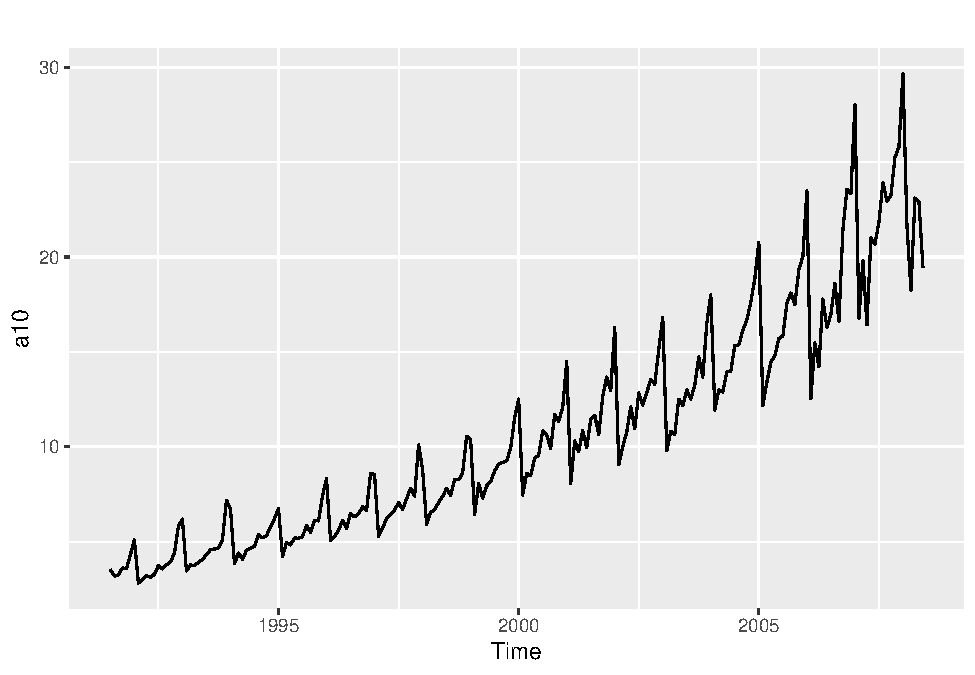
\includegraphics{bookdown-demo_files/figure-latex/unnamed-chunk-2-16.pdf}

\begin{Shaded}
\begin{Highlighting}[]
  \KeywordTok{ggseasonplot}\NormalTok{(a10)}
\end{Highlighting}
\end{Shaded}

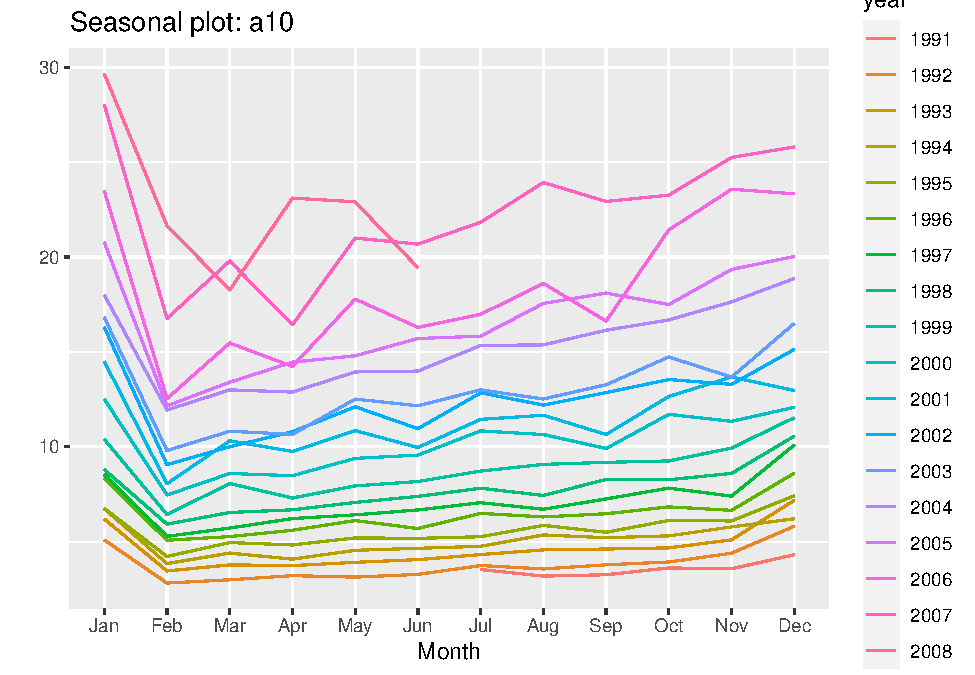
\includegraphics{bookdown-demo_files/figure-latex/unnamed-chunk-2-17.pdf}

\begin{Shaded}
\begin{Highlighting}[]
  \KeywordTok{ggseasonplot}\NormalTok{(a10, }\DataTypeTok{year.labels=}\OtherTok{TRUE}\NormalTok{, }\DataTypeTok{year.labels.left=}\OtherTok{TRUE}\NormalTok{) }\OperatorTok{+}
\StringTok{    }\KeywordTok{ylab}\NormalTok{(}\StringTok{"$ million"}\NormalTok{) }\OperatorTok{+}
\StringTok{    }\KeywordTok{ggtitle}\NormalTok{(}\StringTok{"Seasonal plot: antidiabetic drug sales"}\NormalTok{)}
\end{Highlighting}
\end{Shaded}

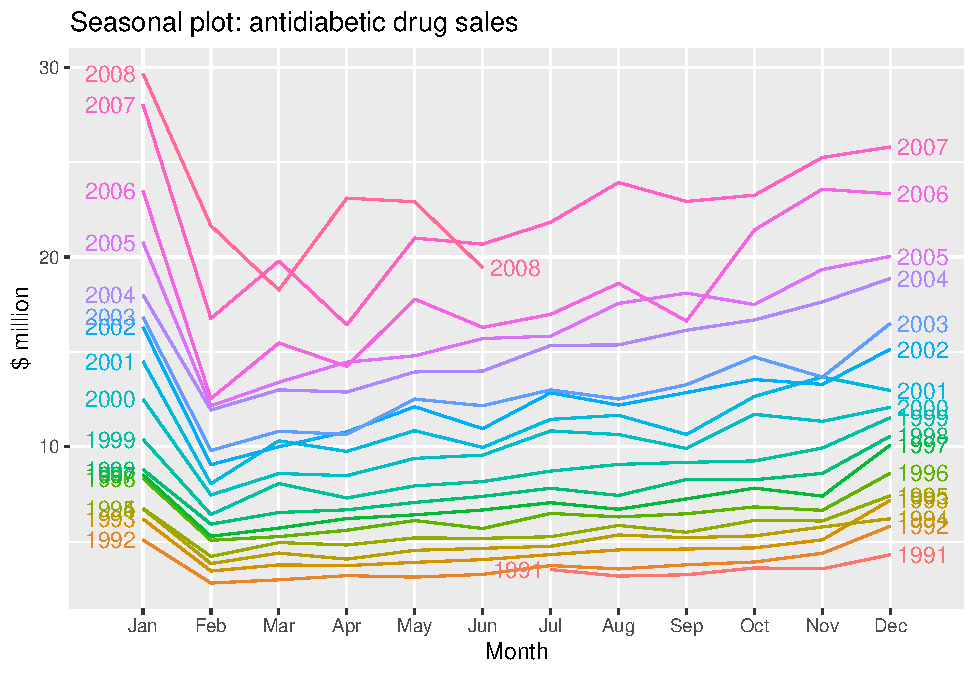
\includegraphics{bookdown-demo_files/figure-latex/unnamed-chunk-2-18.pdf}

\begin{Shaded}
\begin{Highlighting}[]
  \KeywordTok{ggseasonplot}\NormalTok{(a10, }\DataTypeTok{polar=}\OtherTok{TRUE}\NormalTok{) }\OperatorTok{+}\StringTok{ }\KeywordTok{ylab}\NormalTok{(}\StringTok{"$ million"}\NormalTok{)  }
\end{Highlighting}
\end{Shaded}

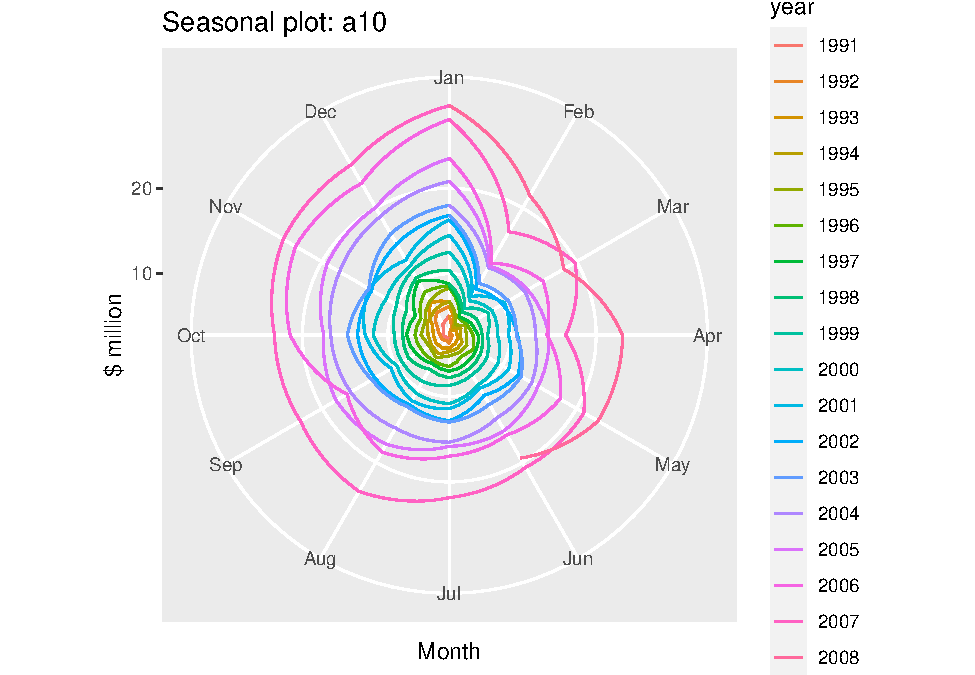
\includegraphics{bookdown-demo_files/figure-latex/unnamed-chunk-2-19.pdf}

\begin{Shaded}
\begin{Highlighting}[]
\CommentTok{# Seasonal subseries plots}
  \KeywordTok{ggsubseriesplot}\NormalTok{(a10) }\OperatorTok{+}\StringTok{ }\KeywordTok{ylab}\NormalTok{(}\StringTok{"$ million"}\NormalTok{) }\OperatorTok{+}
\StringTok{    }\KeywordTok{ggtitle}\NormalTok{(}\StringTok{"Subseries plot: antidiabetic drug sales"}\NormalTok{)}
\end{Highlighting}
\end{Shaded}

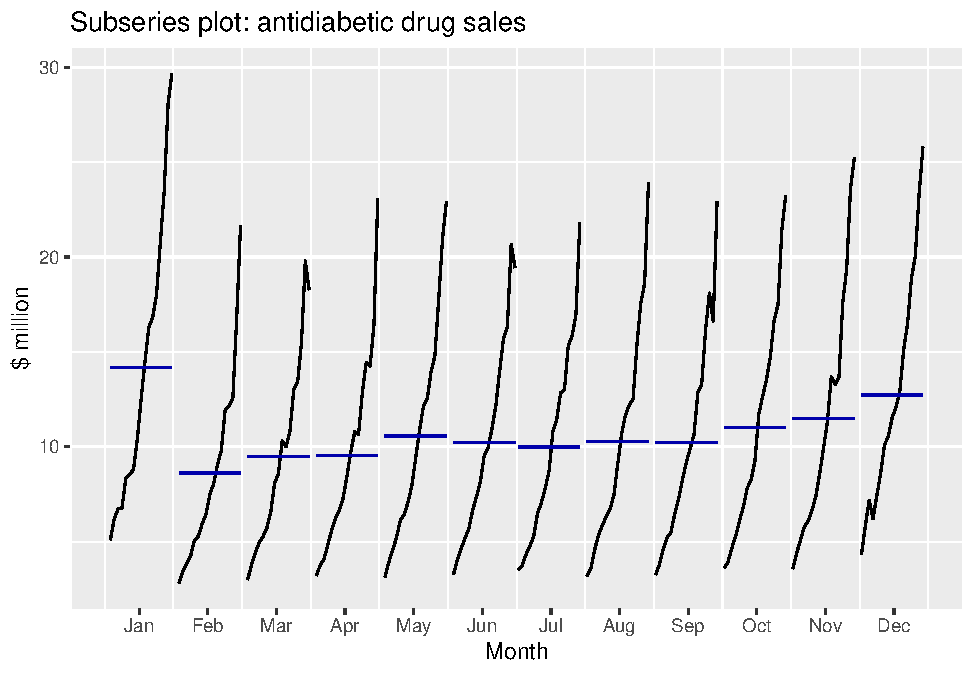
\includegraphics{bookdown-demo_files/figure-latex/unnamed-chunk-2-20.pdf}

\begin{Shaded}
\begin{Highlighting}[]
\CommentTok{# Australian quarterly beer production 1956:Q1 to 2008:Q3.}
  \KeywordTok{autoplot}\NormalTok{(ausbeer)}
\end{Highlighting}
\end{Shaded}

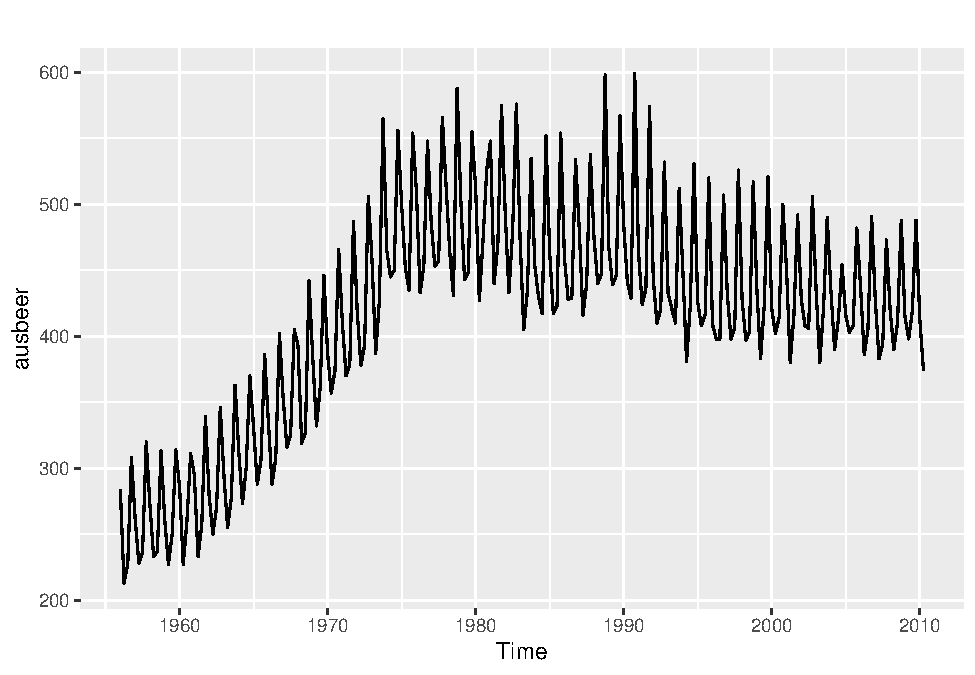
\includegraphics{bookdown-demo_files/figure-latex/unnamed-chunk-2-21.pdf}

\begin{Shaded}
\begin{Highlighting}[]
  \CommentTok{# Take a window of it starting in 1992}
\NormalTok{  beer=}\KeywordTok{window}\NormalTok{(ausbeer,}\DataTypeTok{start=}\DecValTok{1992}\NormalTok{)}
  
  \KeywordTok{autoplot}\NormalTok{(beer)}\OperatorTok{+}\KeywordTok{geom_point}\NormalTok{()}
\end{Highlighting}
\end{Shaded}

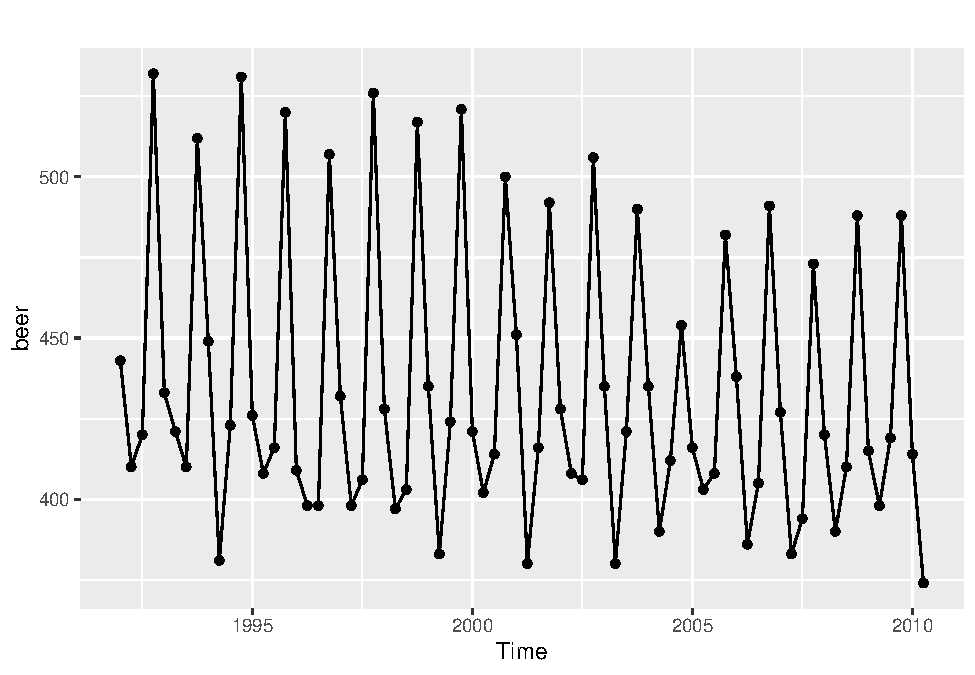
\includegraphics{bookdown-demo_files/figure-latex/unnamed-chunk-2-22.pdf}

\begin{Shaded}
\begin{Highlighting}[]
  \KeywordTok{ggseasonplot}\NormalTok{(beer, }\DataTypeTok{year.labels=}\OtherTok{TRUE}\NormalTok{, }
             \DataTypeTok{year.labels.left=}\OtherTok{TRUE}\NormalTok{)}
\end{Highlighting}
\end{Shaded}

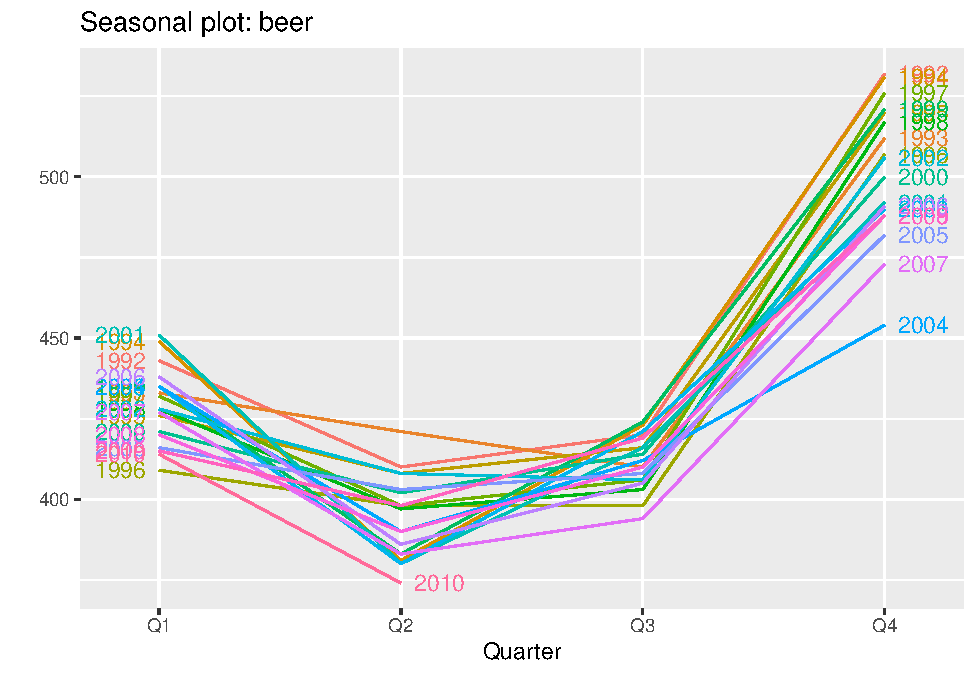
\includegraphics{bookdown-demo_files/figure-latex/unnamed-chunk-2-23.pdf}

\begin{Shaded}
\begin{Highlighting}[]
  \KeywordTok{ggsubseriesplot}\NormalTok{(beer)}\OperatorTok{+}\KeywordTok{ggtitle}\NormalTok{(}\StringTok{"Subseries Plot"}\NormalTok{)}
\end{Highlighting}
\end{Shaded}

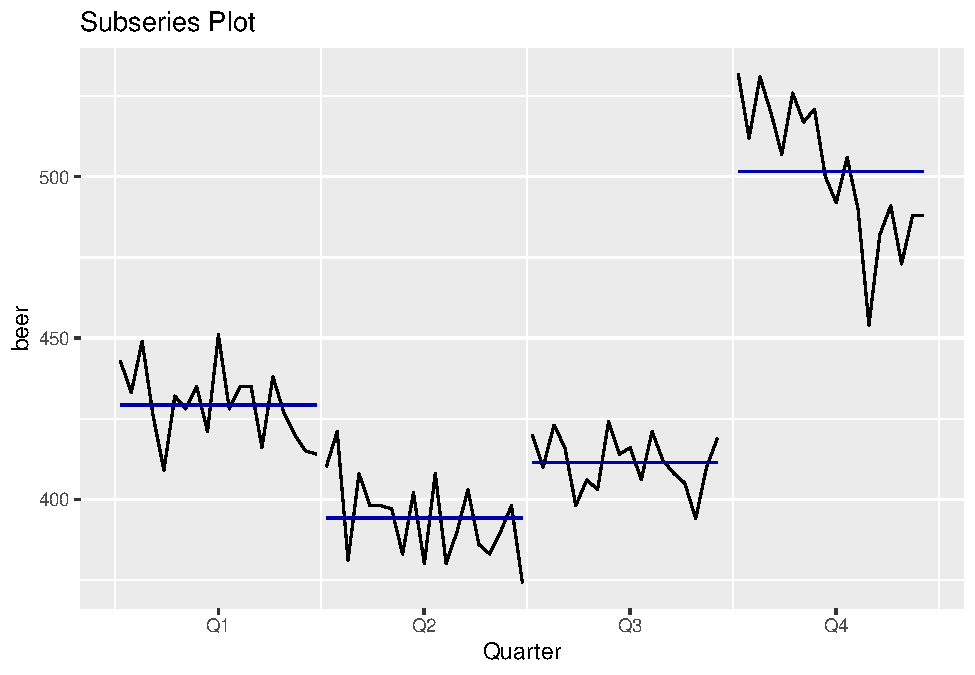
\includegraphics{bookdown-demo_files/figure-latex/unnamed-chunk-2-24.pdf}

\begin{Shaded}
\begin{Highlighting}[]
\CommentTok{# Students to run arrivals code below }
  \CommentTok{# Your turn 1}
\NormalTok{  ?arrivals}
  \KeywordTok{head}\NormalTok{(arrivals)}
\end{Highlighting}
\end{Shaded}

\begin{verbatim}
##          Japan     NZ     UK     US
## 1981 Q1 14.763 49.140 45.266 32.316
## 1981 Q2  9.321 87.467 19.886 23.721
## 1981 Q3 10.166 85.841 24.839 24.533
## 1981 Q4 19.509 61.882 52.264 33.438
## 1982 Q1 17.117 42.045 53.636 33.527
## 1982 Q2 10.617 63.081 34.802 28.366
\end{verbatim}

\begin{Shaded}
\begin{Highlighting}[]
  \KeywordTok{autoplot}\NormalTok{(arrivals)  }
\end{Highlighting}
\end{Shaded}

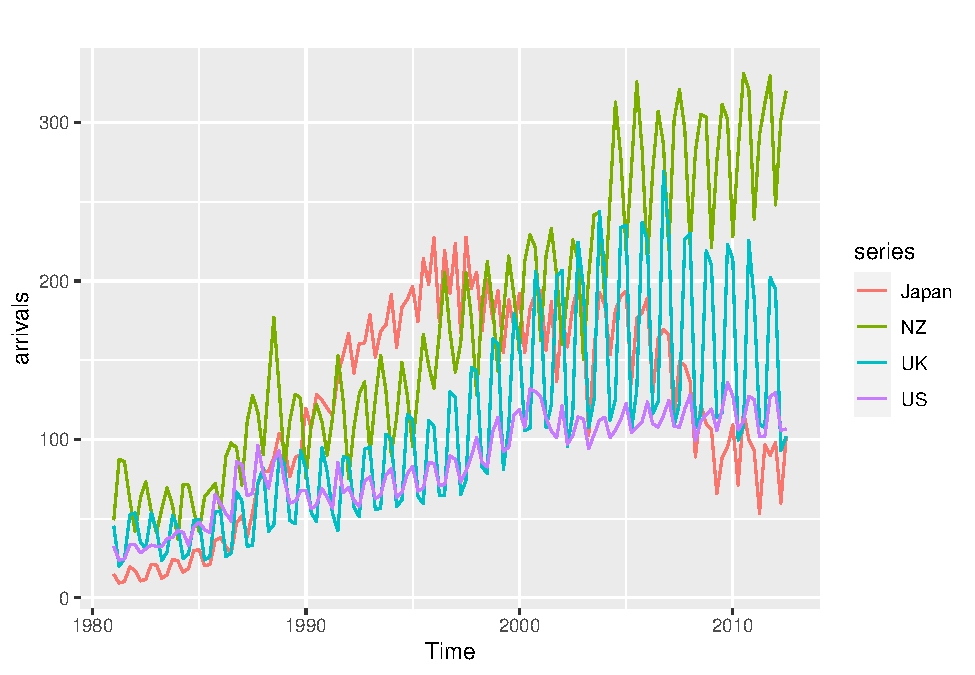
\includegraphics{bookdown-demo_files/figure-latex/unnamed-chunk-2-25.pdf}

\begin{Shaded}
\begin{Highlighting}[]
  \KeywordTok{autoplot}\NormalTok{(arrivals, }\DataTypeTok{facets =} \OtherTok{TRUE}\NormalTok{)  }
\end{Highlighting}
\end{Shaded}

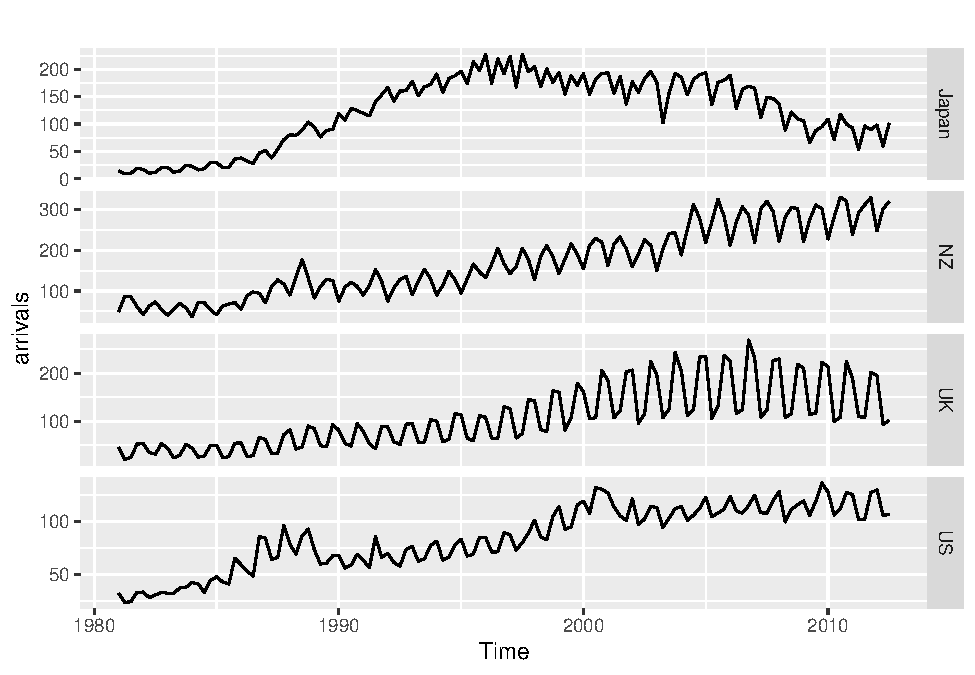
\includegraphics{bookdown-demo_files/figure-latex/unnamed-chunk-2-26.pdf}

\begin{Shaded}
\begin{Highlighting}[]
  \KeywordTok{ggseasonplot}\NormalTok{(arrivals[,}\StringTok{"NZ"}\NormalTok{])}
\end{Highlighting}
\end{Shaded}

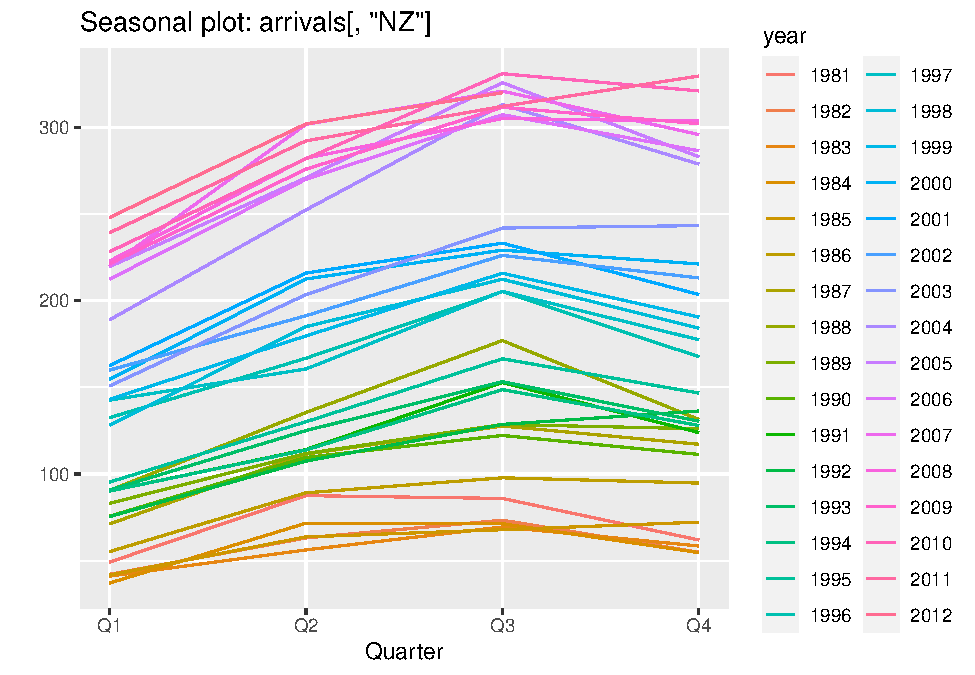
\includegraphics{bookdown-demo_files/figure-latex/unnamed-chunk-2-27.pdf}

\begin{Shaded}
\begin{Highlighting}[]
  \KeywordTok{ggseasonplot}\NormalTok{(arrivals[,}\StringTok{"UK"}\NormalTok{])}
\end{Highlighting}
\end{Shaded}

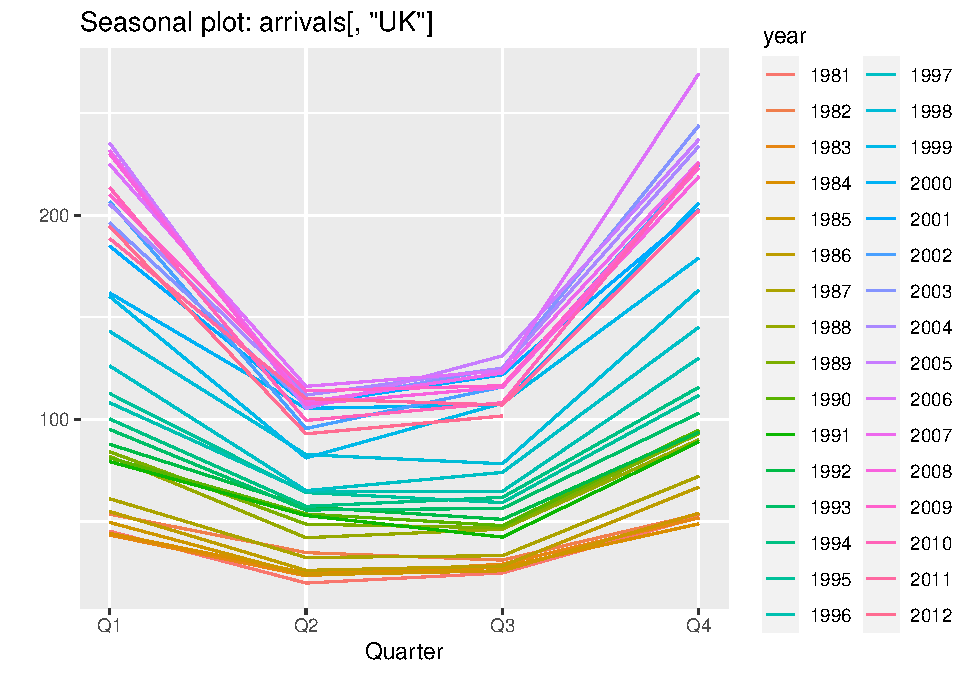
\includegraphics{bookdown-demo_files/figure-latex/unnamed-chunk-2-28.pdf}

\begin{Shaded}
\begin{Highlighting}[]
  \CommentTok{# Plot these together to have a closer look}
\NormalTok{  p1 <-}\StringTok{ }\KeywordTok{ggseasonplot}\NormalTok{(arrivals[,}\StringTok{"NZ"}\NormalTok{])}
\NormalTok{  p2 <-}\StringTok{ }\KeywordTok{ggseasonplot}\NormalTok{(arrivals[,}\StringTok{"UK"}\NormalTok{])}
\NormalTok{  gridExtra}\OperatorTok{::}\KeywordTok{grid.arrange}\NormalTok{(p1,p2,}\DataTypeTok{nrow=}\DecValTok{1}\NormalTok{)}
\end{Highlighting}
\end{Shaded}

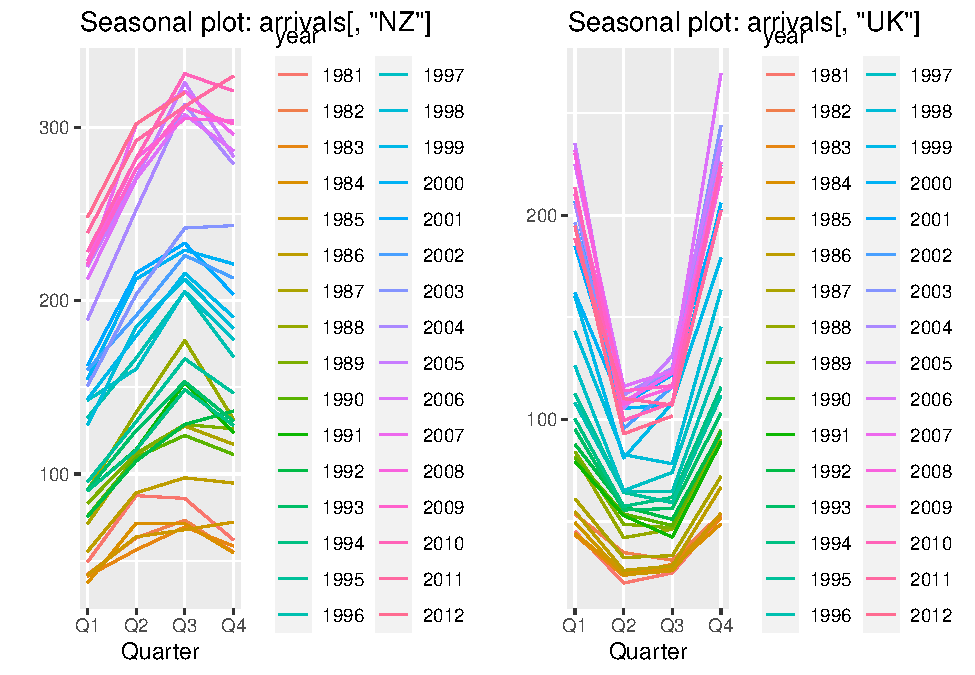
\includegraphics{bookdown-demo_files/figure-latex/unnamed-chunk-2-29.pdf}

\begin{Shaded}
\begin{Highlighting}[]
\CommentTok{#Back to lecture slides}

  \CommentTok{# Time series patterns}
  \KeywordTok{autoplot}\NormalTok{(}\KeywordTok{window}\NormalTok{(elec, }\DataTypeTok{start=}\DecValTok{1980}\NormalTok{)) }\OperatorTok{+}
\StringTok{    }\KeywordTok{ggtitle}\NormalTok{(}\StringTok{"Australian electricity production"}\NormalTok{) }\OperatorTok{+}
\StringTok{    }\KeywordTok{xlab}\NormalTok{(}\StringTok{"Year"}\NormalTok{) }\OperatorTok{+}\StringTok{ }\KeywordTok{ylab}\NormalTok{(}\StringTok{"GWh"}\NormalTok{)}
\end{Highlighting}
\end{Shaded}

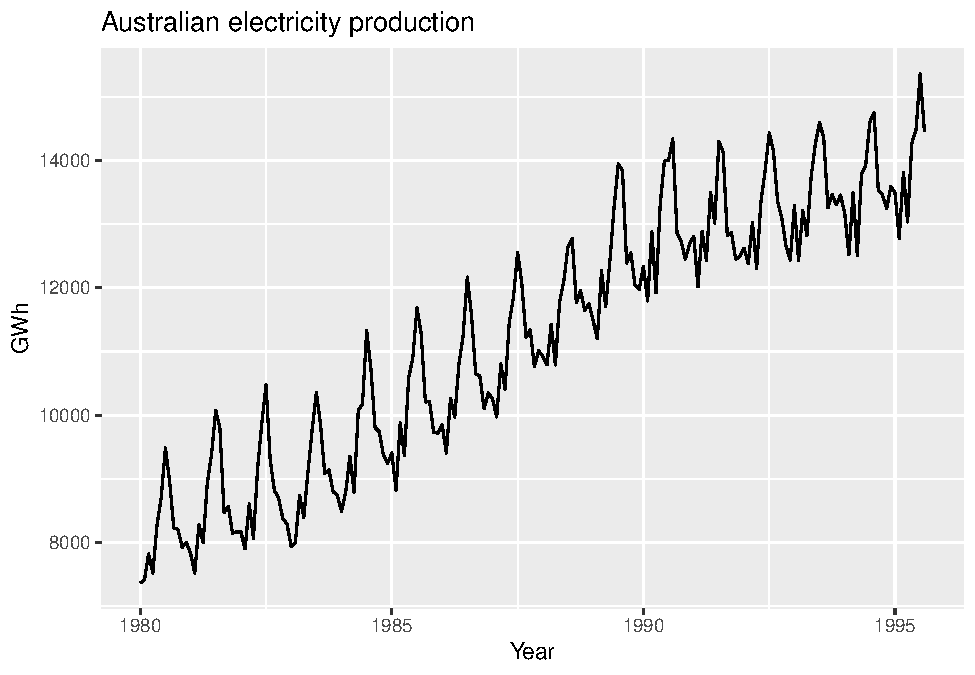
\includegraphics{bookdown-demo_files/figure-latex/unnamed-chunk-2-30.pdf}

\begin{Shaded}
\begin{Highlighting}[]
  \KeywordTok{autoplot}\NormalTok{(bricksq) }\OperatorTok{+}
\StringTok{    }\KeywordTok{ggtitle}\NormalTok{(}\StringTok{"Australian clay brick production"}\NormalTok{) }\OperatorTok{+}
\StringTok{    }\KeywordTok{xlab}\NormalTok{(}\StringTok{"Year"}\NormalTok{) }\OperatorTok{+}\StringTok{ }\KeywordTok{ylab}\NormalTok{(}\StringTok{"million units"}\NormalTok{)}
\end{Highlighting}
\end{Shaded}

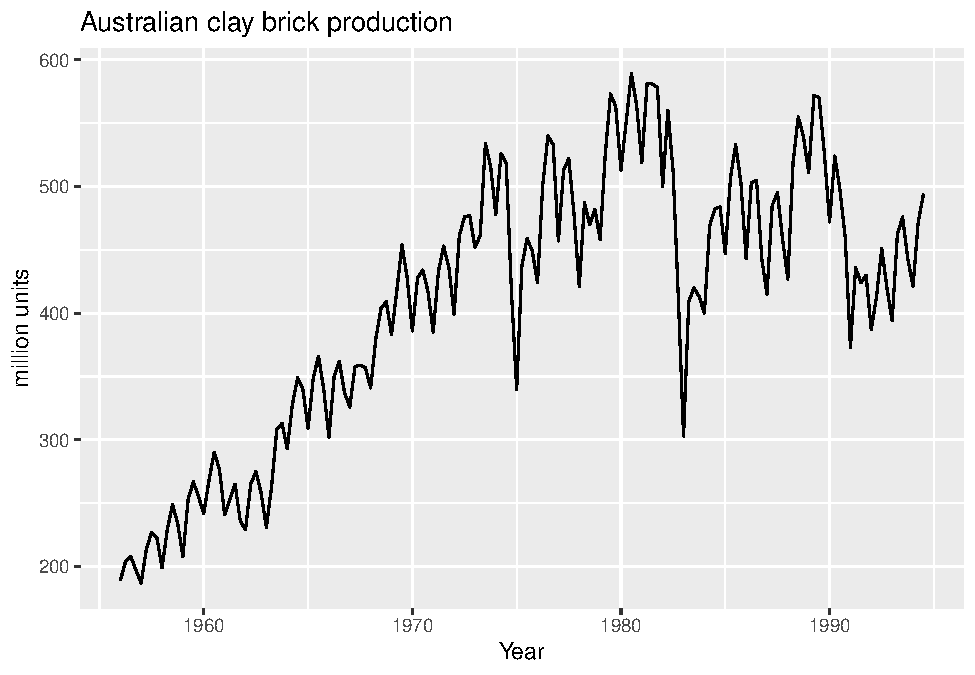
\includegraphics{bookdown-demo_files/figure-latex/unnamed-chunk-2-31.pdf}

\begin{Shaded}
\begin{Highlighting}[]
  \KeywordTok{autoplot}\NormalTok{(hsales) }\OperatorTok{+}
\StringTok{    }\KeywordTok{ggtitle}\NormalTok{(}\StringTok{"Sales of new one-family houses, USA"}\NormalTok{) }\OperatorTok{+}
\StringTok{    }\KeywordTok{xlab}\NormalTok{(}\StringTok{"Year"}\NormalTok{) }\OperatorTok{+}\StringTok{ }\KeywordTok{ylab}\NormalTok{(}\StringTok{"Total sales"}\NormalTok{)}
\end{Highlighting}
\end{Shaded}

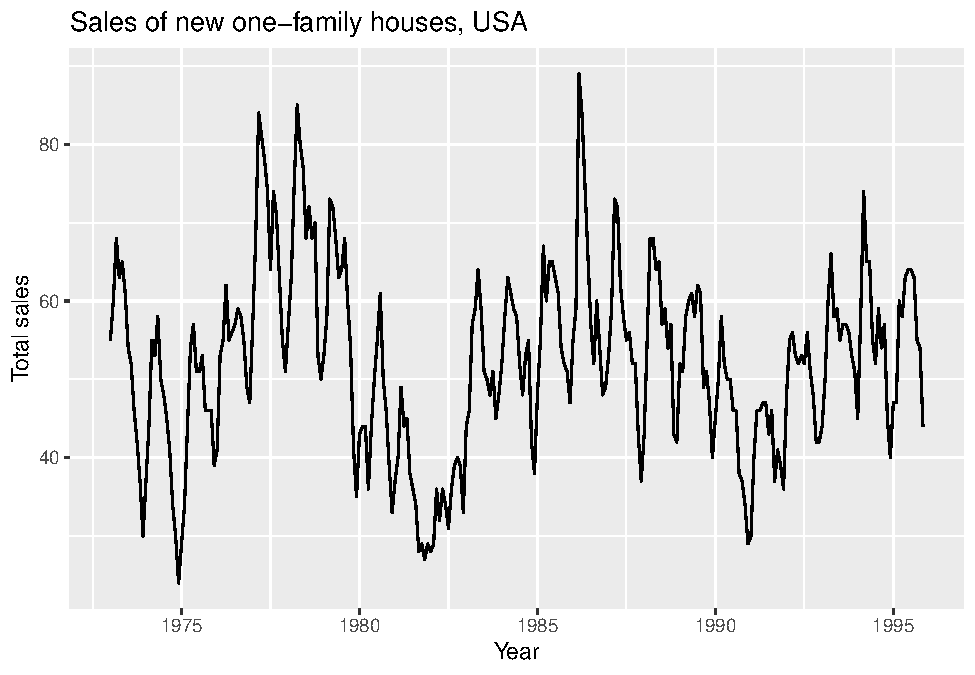
\includegraphics{bookdown-demo_files/figure-latex/unnamed-chunk-2-32.pdf}

\begin{Shaded}
\begin{Highlighting}[]
  \KeywordTok{autoplot}\NormalTok{(ustreas) }\OperatorTok{+}
\StringTok{    }\KeywordTok{ggtitle}\NormalTok{(}\StringTok{"US Treasury Bill Contracts"}\NormalTok{) }\OperatorTok{+}
\StringTok{    }\KeywordTok{xlab}\NormalTok{(}\StringTok{"Day"}\NormalTok{) }\OperatorTok{+}\StringTok{ }\KeywordTok{ylab}\NormalTok{(}\StringTok{"price"}\NormalTok{)}
\end{Highlighting}
\end{Shaded}

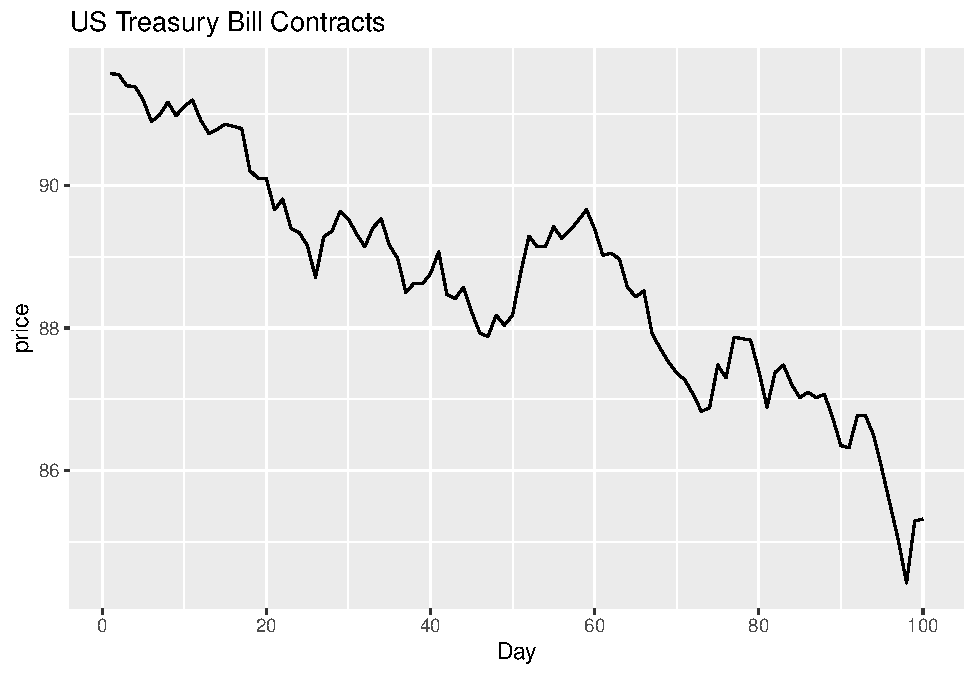
\includegraphics{bookdown-demo_files/figure-latex/unnamed-chunk-2-33.pdf}

\begin{Shaded}
\begin{Highlighting}[]
  \KeywordTok{autoplot}\NormalTok{(lynx) }\OperatorTok{+}
\StringTok{    }\KeywordTok{ggtitle}\NormalTok{(}\StringTok{"Annual Canadian Lynx Trappings"}\NormalTok{) }\OperatorTok{+}
\StringTok{    }\KeywordTok{xlab}\NormalTok{(}\StringTok{"Year"}\NormalTok{) }\OperatorTok{+}\StringTok{ }\KeywordTok{ylab}\NormalTok{(}\StringTok{"Number trapped"}\NormalTok{)}
\end{Highlighting}
\end{Shaded}

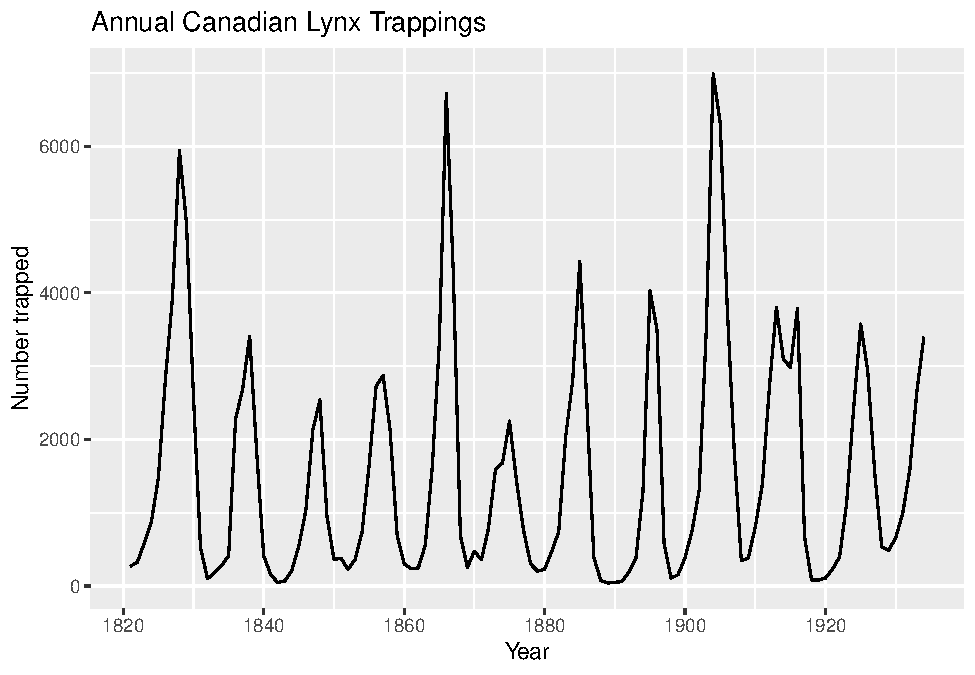
\includegraphics{bookdown-demo_files/figure-latex/unnamed-chunk-2-34.pdf}

\begin{Shaded}
\begin{Highlighting}[]
\CommentTok{#Back to lecture slides}
  
\CommentTok{# Scatterplots}
  \KeywordTok{head}\NormalTok{(motel)}
\end{Highlighting}
\end{Shaded}

\begin{verbatim}
##          Roomnights Takings
## Jan 1980      277.0     7.7
## Feb 1980      260.6     7.5
## Mar 1980      291.6     8.3
## Apr 1980      275.4     7.8
## May 1980      275.3     7.9
## Jun 1980      231.7     6.6
\end{verbatim}

\begin{Shaded}
\begin{Highlighting}[]
    \KeywordTok{autoplot}\NormalTok{(motel[,}\DecValTok{2}\OperatorTok{:}\DecValTok{1}\NormalTok{]}\OperatorTok{/}\DecValTok{1000}\NormalTok{, }\DataTypeTok{facet=}\OtherTok{TRUE}\NormalTok{) }\OperatorTok{+}
\StringTok{    }\KeywordTok{xlab}\NormalTok{(}\StringTok{"Year"}\NormalTok{) }\OperatorTok{+}\StringTok{ }\KeywordTok{ylab}\NormalTok{(}\StringTok{""}\NormalTok{) }\OperatorTok{+}
\StringTok{    }\KeywordTok{ggtitle}\NormalTok{(}\StringTok{"Total monthly accommodation: Victoria, Australia"}\NormalTok{)}
\end{Highlighting}
\end{Shaded}

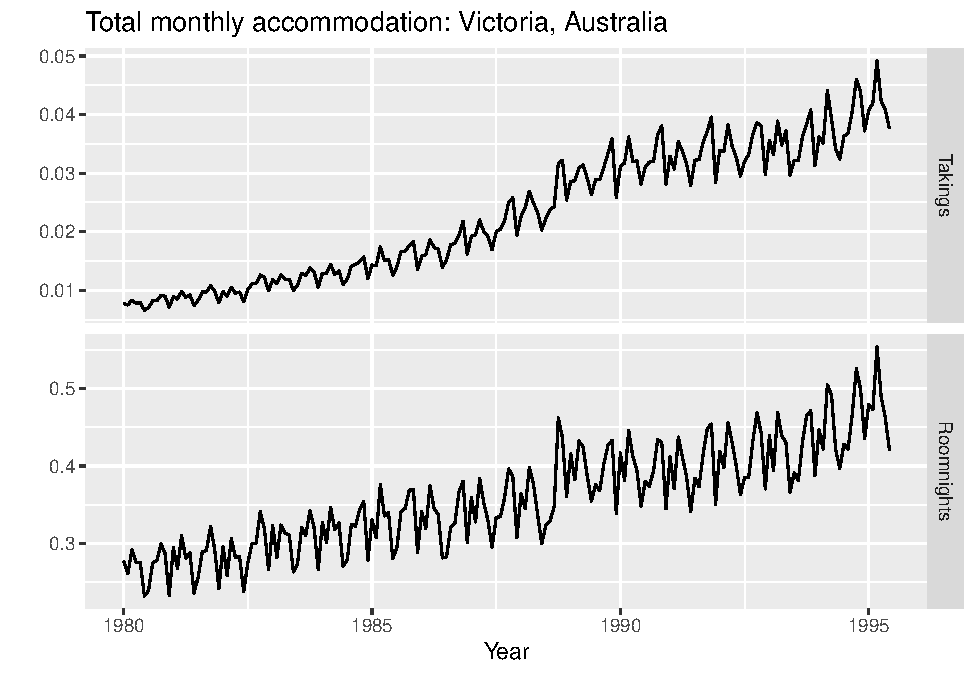
\includegraphics{bookdown-demo_files/figure-latex/unnamed-chunk-2-35.pdf}

\begin{Shaded}
\begin{Highlighting}[]
    \CommentTok{# See what happens without the facet=TRUE argument}
    \KeywordTok{autoplot}\NormalTok{(motel[,}\DecValTok{2}\OperatorTok{:}\DecValTok{1}\NormalTok{]}\OperatorTok{/}\DecValTok{1000}\NormalTok{)}
\end{Highlighting}
\end{Shaded}

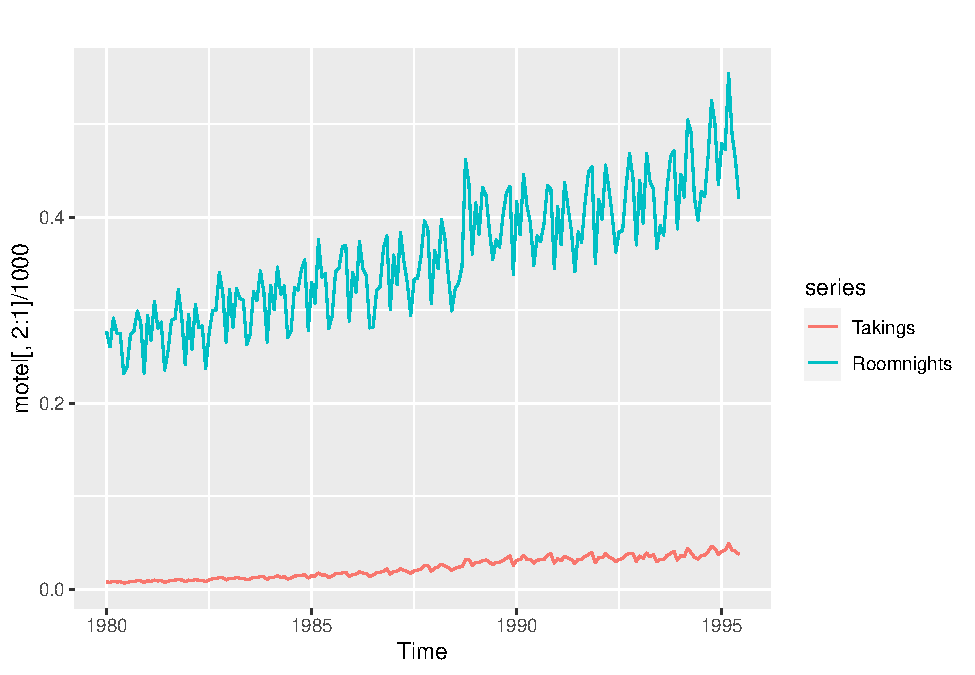
\includegraphics{bookdown-demo_files/figure-latex/unnamed-chunk-2-36.pdf}

\begin{Shaded}
\begin{Highlighting}[]
    \CommentTok{# doesn't make much sense because of the differences in scale}
    
  \KeywordTok{qplot}\NormalTok{(Roomnights}\OperatorTok{/}\DecValTok{1000}\NormalTok{, Takings}\OperatorTok{/}\DecValTok{1000}\NormalTok{, }\DataTypeTok{data=}\KeywordTok{as.data.frame}\NormalTok{(motel)) }\OperatorTok{+}
\StringTok{    }\KeywordTok{ylab}\NormalTok{(}\StringTok{"Takings ($million)"}\NormalTok{) }\OperatorTok{+}\StringTok{ }\KeywordTok{xlab}\NormalTok{(}\StringTok{"Room nights (thousands)"}\NormalTok{)}
\end{Highlighting}
\end{Shaded}

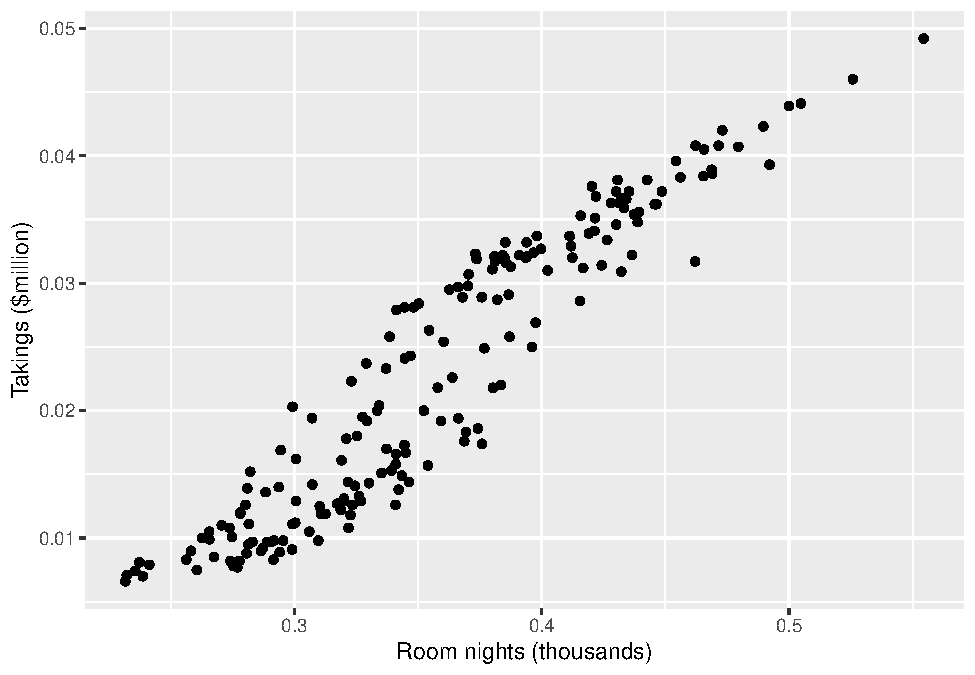
\includegraphics{bookdown-demo_files/figure-latex/unnamed-chunk-2-37.pdf}

\begin{Shaded}
\begin{Highlighting}[]
  \KeywordTok{head}\NormalTok{(motel)}
\end{Highlighting}
\end{Shaded}

\begin{verbatim}
##          Roomnights Takings
## Jan 1980      277.0     7.7
## Feb 1980      260.6     7.5
## Mar 1980      291.6     8.3
## Apr 1980      275.4     7.8
## May 1980      275.3     7.9
## Jun 1980      231.7     6.6
\end{verbatim}

\begin{Shaded}
\begin{Highlighting}[]
  \KeywordTok{head}\NormalTok{(}\KeywordTok{as.data.frame}\NormalTok{(motel))}
\end{Highlighting}
\end{Shaded}

\begin{verbatim}
##   Roomnights Takings
## 1      277.0     7.7
## 2      260.6     7.5
## 3      291.6     8.3
## 4      275.4     7.8
## 5      275.3     7.9
## 6      231.7     6.6
\end{verbatim}

\begin{Shaded}
\begin{Highlighting}[]
\CommentTok{#Back to slides}
  
\CommentTok{# Lag plots and autocorrelation }
\NormalTok{  beer <-}\StringTok{ }\KeywordTok{window}\NormalTok{(ausbeer, }\DataTypeTok{start=}\DecValTok{1992}\NormalTok{)}
  \KeywordTok{gglagplot}\NormalTok{(beer, }\DataTypeTok{lags=}\DecValTok{9}\NormalTok{)}
\end{Highlighting}
\end{Shaded}

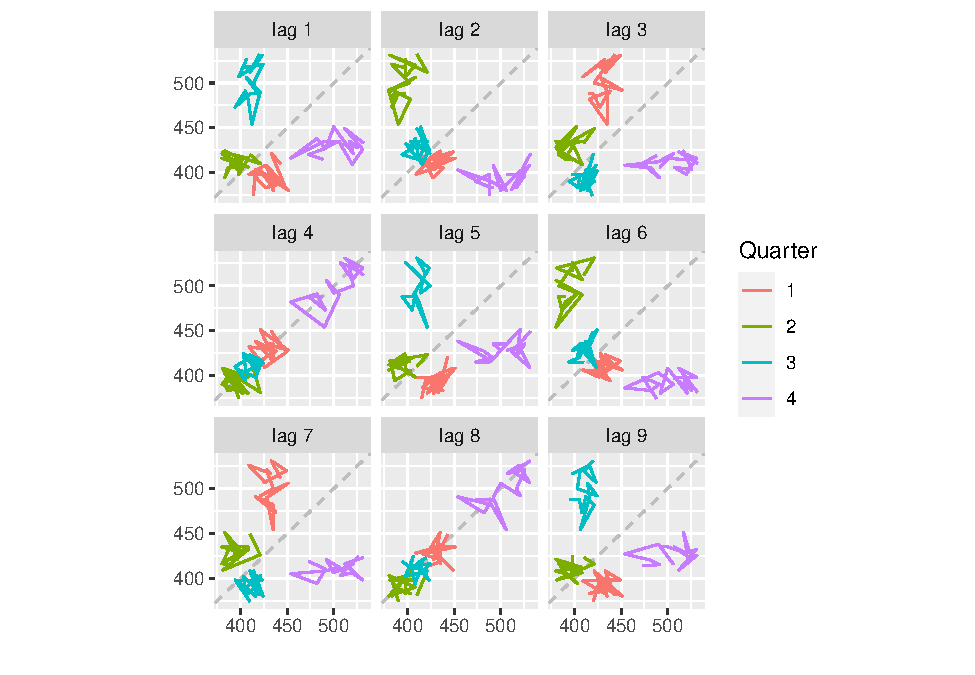
\includegraphics{bookdown-demo_files/figure-latex/unnamed-chunk-2-38.pdf}

\begin{Shaded}
\begin{Highlighting}[]
  \CommentTok{# What does the 'do.lines=FALSE' do?}
  \KeywordTok{gglagplot}\NormalTok{(beer, }\DataTypeTok{lags=}\DecValTok{9}\NormalTok{, }\DataTypeTok{do.lines=}\OtherTok{FALSE}\NormalTok{)}
\end{Highlighting}
\end{Shaded}

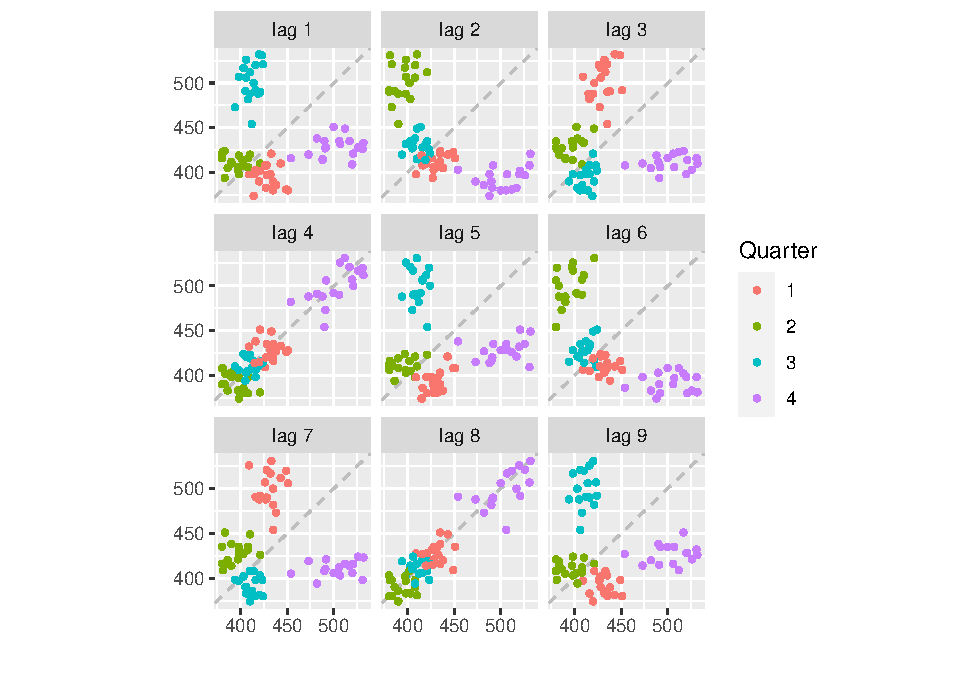
\includegraphics{bookdown-demo_files/figure-latex/unnamed-chunk-2-39.pdf}

\begin{Shaded}
\begin{Highlighting}[]
\CommentTok{# ACF}
  \KeywordTok{ggAcf}\NormalTok{(beer) }\CommentTok{#from forecast package}
\end{Highlighting}
\end{Shaded}

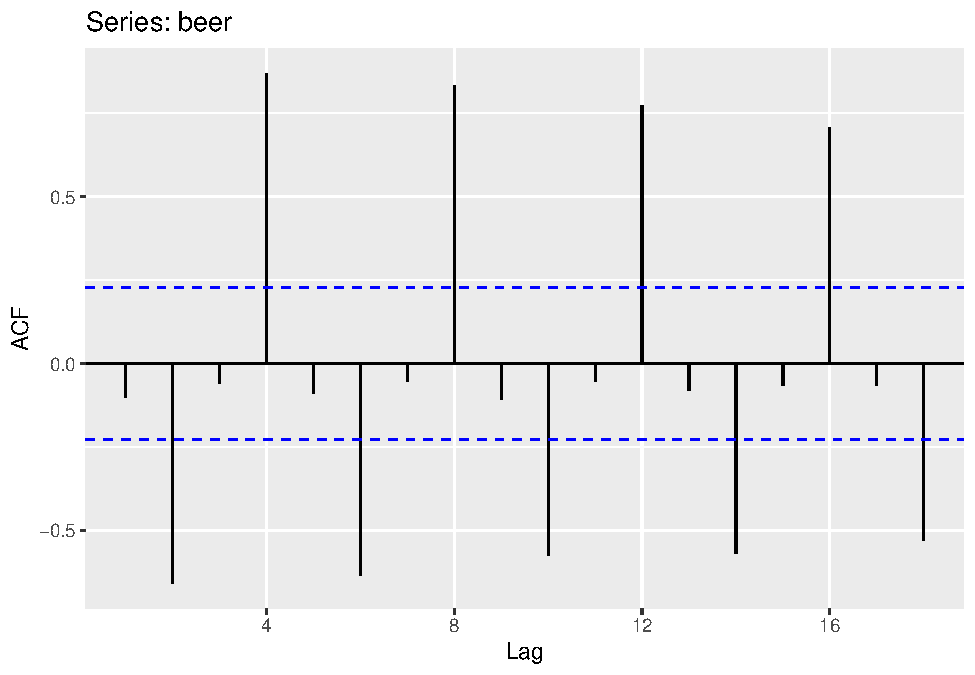
\includegraphics{bookdown-demo_files/figure-latex/unnamed-chunk-2-40.pdf}

\begin{Shaded}
\begin{Highlighting}[]
\NormalTok{  r<-}\KeywordTok{ggAcf}\NormalTok{(beer)}
  \KeywordTok{attributes}\NormalTok{(r)  }
\end{Highlighting}
\end{Shaded}

\begin{verbatim}
## $names
## [1] "data"        "layers"      "scales"      "mapping"     "theme"      
## [6] "coordinates" "facet"       "plot_env"    "labels"     
## 
## $class
## [1] "gg"     "ggplot"
\end{verbatim}

\begin{Shaded}
\begin{Highlighting}[]
\NormalTok{  r}\OperatorTok{$}\NormalTok{data}
\end{Highlighting}
\end{Shaded}

\begin{verbatim}
##    Var2 Var3        Freq lag
## 2     A    A -0.10190904   1
## 3     A    A -0.65661956   2
## 4     A    A -0.06027634   3
## 5     A    A  0.86852930   4
## 6     A    A -0.08915021   5
## 7     A    A -0.63513179   6
## 8     A    A -0.05416215   7
## 9     A    A  0.83224495   8
## 10    A    A -0.10787557   9
## 11    A    A -0.57419959  10
## 12    A    A -0.05460320  11
## 13    A    A  0.77379390  12
## 14    A    A -0.08019609  13
## 15    A    A -0.56805745  14
## 16    A    A -0.06626388  15
## 17    A    A  0.70642954  16
## 18    A    A -0.06535949  17
## 19    A    A -0.52825861  18
\end{verbatim}

\begin{Shaded}
\begin{Highlighting}[]
\NormalTok{  r}\OperatorTok{$}\NormalTok{data}\OperatorTok{$}\NormalTok{Freq}
\end{Highlighting}
\end{Shaded}

\begin{verbatim}
##  [1] -0.10190904 -0.65661956 -0.06027634  0.86852930 -0.08915021 -0.63513179
##  [7] -0.05416215  0.83224495 -0.10787557 -0.57419959 -0.05460320  0.77379390
## [13] -0.08019609 -0.56805745 -0.06626388  0.70642954 -0.06535949 -0.52825861
\end{verbatim}

\begin{Shaded}
\begin{Highlighting}[]
\NormalTok{  r}\OperatorTok{$}\NormalTok{data}\OperatorTok{$}\NormalTok{Freq[}\DecValTok{4}\NormalTok{]}
\end{Highlighting}
\end{Shaded}

\begin{verbatim}
## [1] 0.8685293
\end{verbatim}

\begin{Shaded}
\begin{Highlighting}[]
\CommentTok{# Back to slides}

  \KeywordTok{autoplot}\NormalTok{(goog)}
\end{Highlighting}
\end{Shaded}

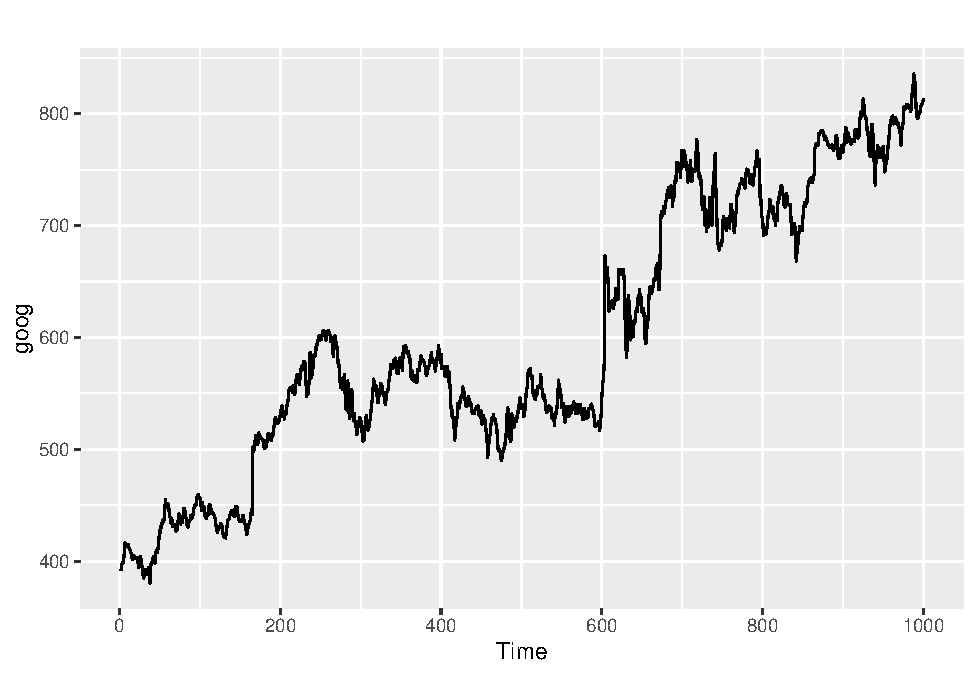
\includegraphics{bookdown-demo_files/figure-latex/unnamed-chunk-2-41.pdf}

\begin{Shaded}
\begin{Highlighting}[]
  \KeywordTok{ggAcf}\NormalTok{(goog, }\DataTypeTok{lag.max=}\DecValTok{100}\NormalTok{)}
\end{Highlighting}
\end{Shaded}

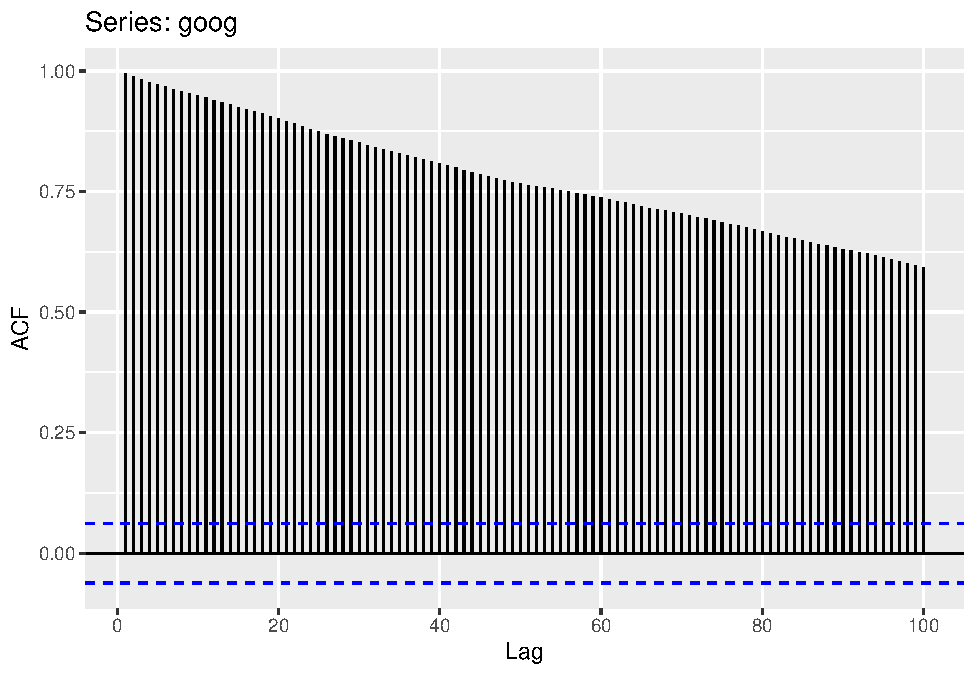
\includegraphics{bookdown-demo_files/figure-latex/unnamed-chunk-2-42.pdf}

\begin{Shaded}
\begin{Highlighting}[]
\NormalTok{  elec2 <-}\StringTok{ }\KeywordTok{window}\NormalTok{(elec, }\DataTypeTok{start=}\DecValTok{1980}\NormalTok{)}
  \KeywordTok{autoplot}\NormalTok{(elec2)}
\end{Highlighting}
\end{Shaded}

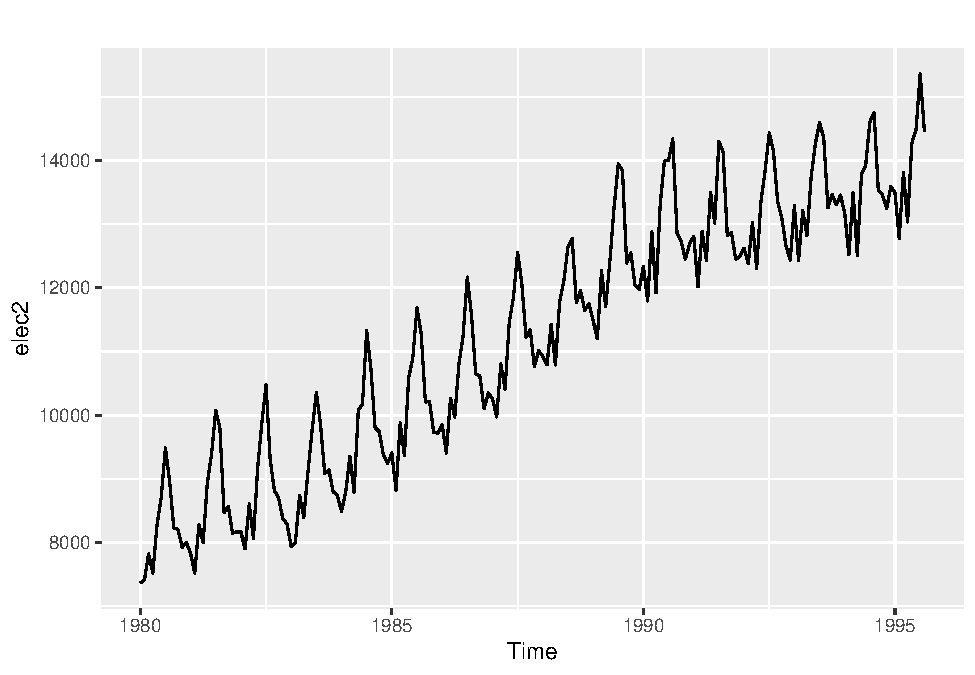
\includegraphics{bookdown-demo_files/figure-latex/unnamed-chunk-2-43.pdf}

\begin{Shaded}
\begin{Highlighting}[]
  \KeywordTok{ggAcf}\NormalTok{(elec2, }\DataTypeTok{lag.max=}\DecValTok{48}\NormalTok{)}
\end{Highlighting}
\end{Shaded}

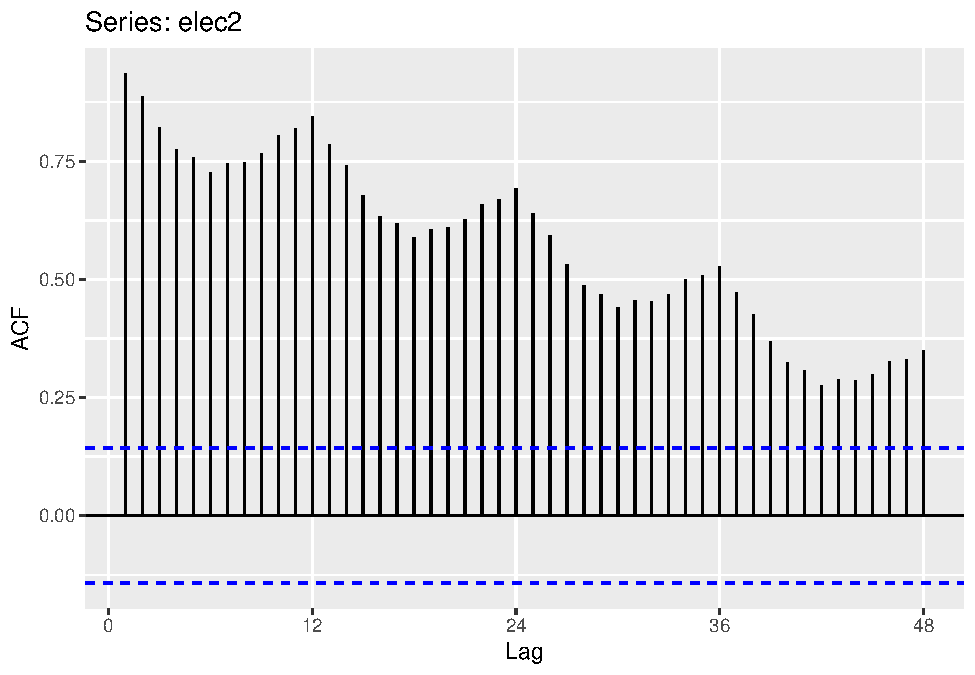
\includegraphics{bookdown-demo_files/figure-latex/unnamed-chunk-2-44.pdf}

\begin{Shaded}
\begin{Highlighting}[]
\CommentTok{# Students to run }
\NormalTok{  ?usdeaths}
  \KeywordTok{autoplot}\NormalTok{(usdeaths)}
\end{Highlighting}
\end{Shaded}

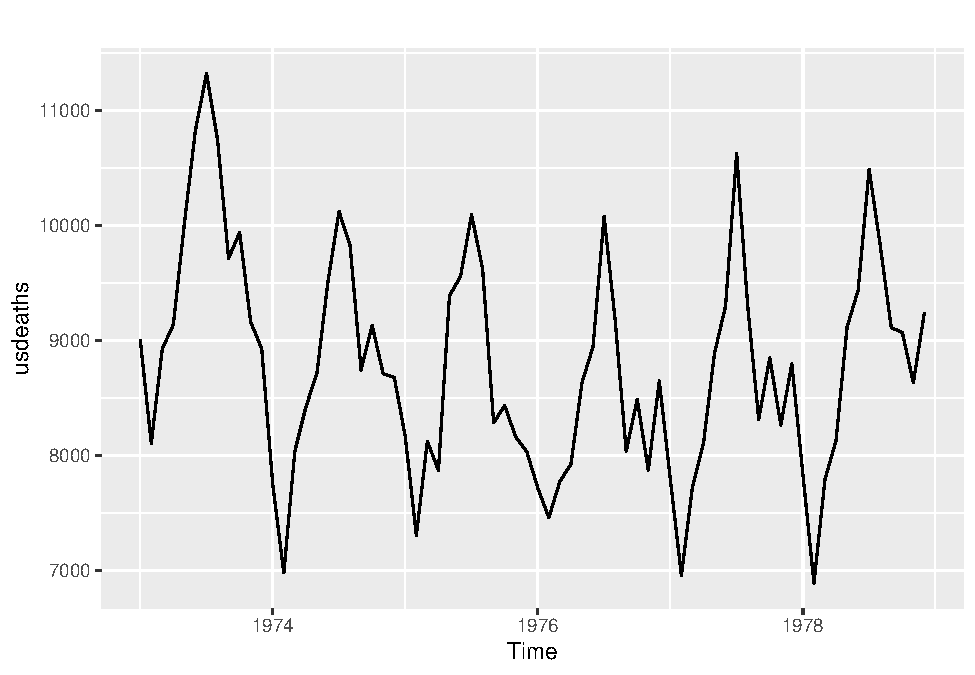
\includegraphics{bookdown-demo_files/figure-latex/unnamed-chunk-2-45.pdf}

\begin{Shaded}
\begin{Highlighting}[]
  \KeywordTok{ggseasonplot}\NormalTok{(usdeaths)}
\end{Highlighting}
\end{Shaded}

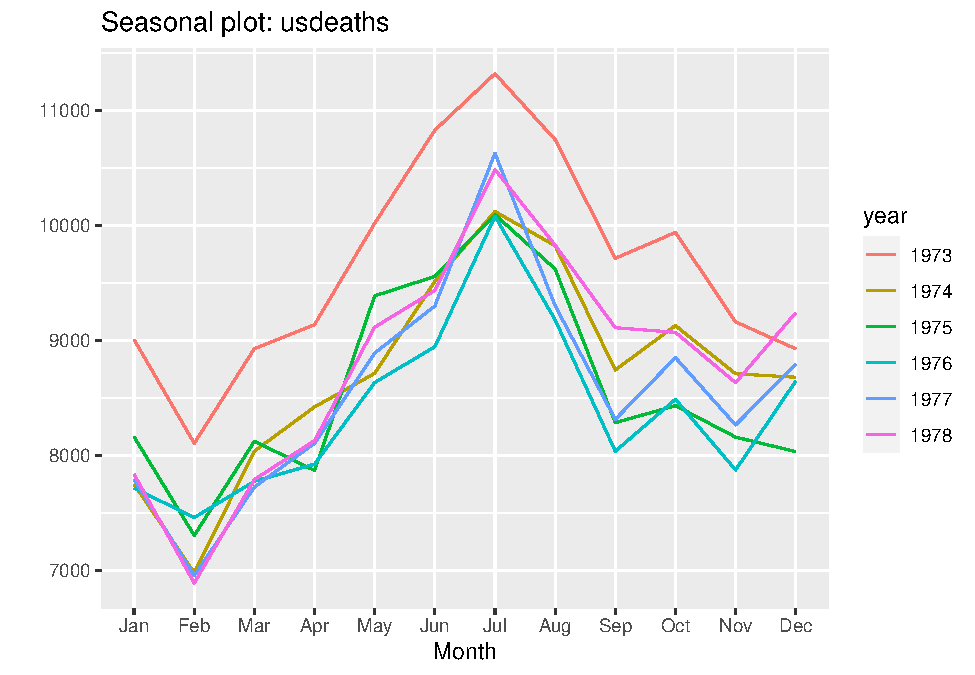
\includegraphics{bookdown-demo_files/figure-latex/unnamed-chunk-2-46.pdf}

\begin{Shaded}
\begin{Highlighting}[]
  \KeywordTok{gglagplot}\NormalTok{(usdeaths)}
\end{Highlighting}
\end{Shaded}

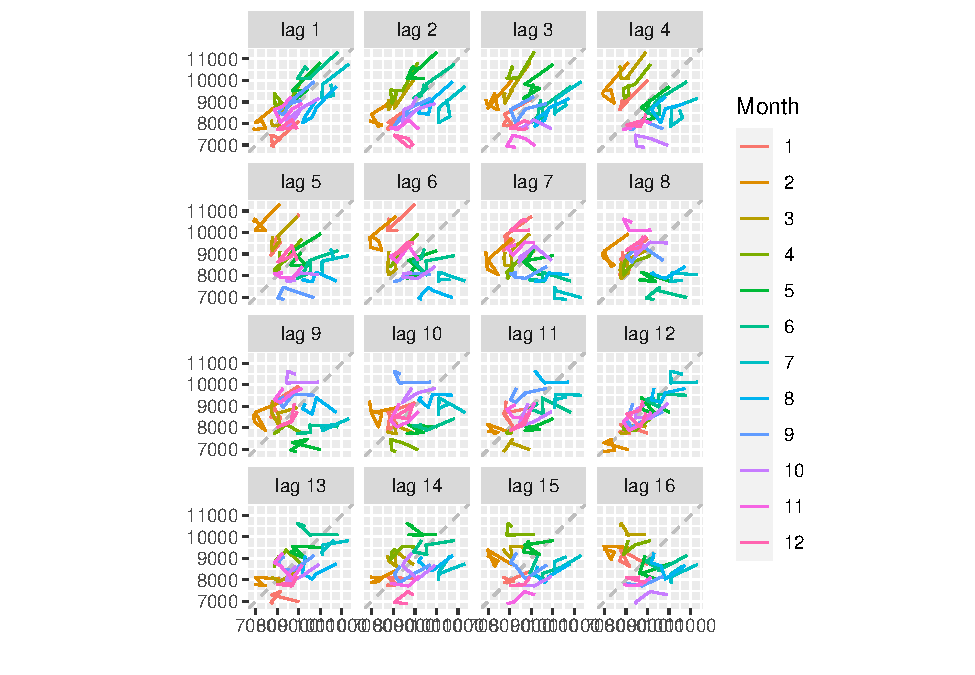
\includegraphics{bookdown-demo_files/figure-latex/unnamed-chunk-2-47.pdf}

\begin{Shaded}
\begin{Highlighting}[]
  \KeywordTok{ggAcf}\NormalTok{(usdeaths)}
\end{Highlighting}
\end{Shaded}

\includegraphics{bookdown-demo_files/figure-latex/unnamed-chunk-2-48.pdf}

\begin{Shaded}
\begin{Highlighting}[]
\NormalTok{  ?sunspotarea}
  \KeywordTok{autoplot}\NormalTok{(sunspotarea)}
\end{Highlighting}
\end{Shaded}

\includegraphics{bookdown-demo_files/figure-latex/unnamed-chunk-2-49.pdf}

\begin{Shaded}
\begin{Highlighting}[]
  \KeywordTok{gglagplot}\NormalTok{(sunspotarea, }\DataTypeTok{do.lines=}\OtherTok{FALSE}\NormalTok{)  }
\end{Highlighting}
\end{Shaded}

\includegraphics{bookdown-demo_files/figure-latex/unnamed-chunk-2-50.pdf}

\begin{Shaded}
\begin{Highlighting}[]
  \KeywordTok{ggAcf}\NormalTok{(sunspotarea)}
\end{Highlighting}
\end{Shaded}

\includegraphics{bookdown-demo_files/figure-latex/unnamed-chunk-2-51.pdf}

\begin{Shaded}
\begin{Highlighting}[]
\CommentTok{# bAck to slides.}

\CommentTok{# White noise}
  
  \CommentTok{# Set the seed for the random number generator in R}
  \CommentTok{# This guarantees the same random numbers every time}
  
  \KeywordTok{set.seed}\NormalTok{(}\DecValTok{0}\NormalTok{) }
\NormalTok{  wn <-}\StringTok{ }\KeywordTok{ts}\NormalTok{(}\KeywordTok{rnorm}\NormalTok{(}\DecValTok{36}\NormalTok{)) }\CommentTok{#rnorm(n, mean = 0, sd = 1)}
  \KeywordTok{autoplot}\NormalTok{(wn)}\OperatorTok{+}\KeywordTok{ggtitle}\NormalTok{(}\StringTok{"White noise"}\NormalTok{)}
\end{Highlighting}
\end{Shaded}

\includegraphics{bookdown-demo_files/figure-latex/unnamed-chunk-2-52.pdf}

\begin{Shaded}
\begin{Highlighting}[]
  \KeywordTok{ggAcf}\NormalTok{(wn)}
\end{Highlighting}
\end{Shaded}

\includegraphics{bookdown-demo_files/figure-latex/unnamed-chunk-2-53.pdf}

\begin{Shaded}
\begin{Highlighting}[]
  \KeywordTok{set.seed}\NormalTok{(}\DecValTok{34}\NormalTok{) }
\NormalTok{  wn <-}\StringTok{ }\KeywordTok{ts}\NormalTok{(}\KeywordTok{rnorm}\NormalTok{(}\DecValTok{36}\NormalTok{)) }\CommentTok{#rnorm(n, mean = 0, sd = 1)}
  \KeywordTok{autoplot}\NormalTok{(wn)}\OperatorTok{+}\KeywordTok{ggtitle}\NormalTok{(}\StringTok{"White noise"}\NormalTok{)}
\end{Highlighting}
\end{Shaded}

\includegraphics{bookdown-demo_files/figure-latex/unnamed-chunk-2-54.pdf}

\begin{Shaded}
\begin{Highlighting}[]
  \KeywordTok{ggAcf}\NormalTok{(wn)}
\end{Highlighting}
\end{Shaded}

\includegraphics{bookdown-demo_files/figure-latex/unnamed-chunk-2-55.pdf}

\begin{Shaded}
\begin{Highlighting}[]
  \KeywordTok{set.seed}\NormalTok{(}\DecValTok{0}\NormalTok{) }
\NormalTok{  wn1=}\KeywordTok{ts}\NormalTok{(}\KeywordTok{rnorm}\NormalTok{(}\DecValTok{3600}\NormalTok{,}\DataTypeTok{mean=}\DecValTok{100}\NormalTok{,}\DataTypeTok{sd=}\DecValTok{100}\NormalTok{))}
  \KeywordTok{autoplot}\NormalTok{(wn1)}
\end{Highlighting}
\end{Shaded}

\includegraphics{bookdown-demo_files/figure-latex/unnamed-chunk-2-56.pdf}

\begin{Shaded}
\begin{Highlighting}[]
  \KeywordTok{ggAcf}\NormalTok{(wn1) }\CommentTok{#lag.max}
\end{Highlighting}
\end{Shaded}

\includegraphics{bookdown-demo_files/figure-latex/unnamed-chunk-2-57.pdf}

\begin{Shaded}
\begin{Highlighting}[]
  \KeywordTok{set.seed}\NormalTok{(}\DecValTok{34}\NormalTok{) }
\NormalTok{  wn1=}\KeywordTok{ts}\NormalTok{(}\KeywordTok{rnorm}\NormalTok{(}\DecValTok{3600}\NormalTok{,}\DataTypeTok{mean=}\DecValTok{100}\NormalTok{,}\DataTypeTok{sd=}\DecValTok{100}\NormalTok{))}
  \KeywordTok{autoplot}\NormalTok{(wn1)}
\end{Highlighting}
\end{Shaded}

\includegraphics{bookdown-demo_files/figure-latex/unnamed-chunk-2-58.pdf}

\begin{Shaded}
\begin{Highlighting}[]
  \KeywordTok{ggAcf}\NormalTok{(wn1)}
\end{Highlighting}
\end{Shaded}

\includegraphics{bookdown-demo_files/figure-latex/unnamed-chunk-2-59.pdf}

\begin{Shaded}
\begin{Highlighting}[]
\CommentTok{# Back to slides}
\CommentTok{# Pigs}
\NormalTok{  pigs2 <-}\StringTok{ }\KeywordTok{window}\NormalTok{(pigs, }\DataTypeTok{start=}\DecValTok{1990}\NormalTok{)}
  \KeywordTok{autoplot}\NormalTok{(pigs2) }\OperatorTok{+}
\StringTok{    }\KeywordTok{xlab}\NormalTok{(}\StringTok{"Year"}\NormalTok{) }\OperatorTok{+}\StringTok{ }\KeywordTok{ylab}\NormalTok{(}\StringTok{"thousands"}\NormalTok{) }\OperatorTok{+}
\StringTok{    }\KeywordTok{ggtitle}\NormalTok{(}\StringTok{"Number of pigs slaughtered in Victoria"}\NormalTok{)}
\end{Highlighting}
\end{Shaded}

\includegraphics{bookdown-demo_files/figure-latex/unnamed-chunk-2-60.pdf}

\begin{Shaded}
\begin{Highlighting}[]
  \KeywordTok{ggAcf}\NormalTok{(pigs2)}
\end{Highlighting}
\end{Shaded}

\includegraphics{bookdown-demo_files/figure-latex/unnamed-chunk-2-61.pdf}

\begin{Shaded}
\begin{Highlighting}[]
\CommentTok{# Your turn 2}
  \KeywordTok{autoplot}\NormalTok{(hsales)}
\end{Highlighting}
\end{Shaded}

\includegraphics{bookdown-demo_files/figure-latex/unnamed-chunk-2-62.pdf}

\begin{Shaded}
\begin{Highlighting}[]
  \KeywordTok{ggseasonplot}\NormalTok{(hsales)}
\end{Highlighting}
\end{Shaded}

\includegraphics{bookdown-demo_files/figure-latex/unnamed-chunk-2-63.pdf}

\begin{Shaded}
\begin{Highlighting}[]
  \KeywordTok{ggsubseriesplot}\NormalTok{(hsales)}
\end{Highlighting}
\end{Shaded}

\includegraphics{bookdown-demo_files/figure-latex/unnamed-chunk-2-64.pdf}

\begin{Shaded}
\begin{Highlighting}[]
  \KeywordTok{gglagplot}\NormalTok{(hsales,}\DataTypeTok{do.lines=}\OtherTok{FALSE}\NormalTok{)}
\end{Highlighting}
\end{Shaded}

\includegraphics{bookdown-demo_files/figure-latex/unnamed-chunk-2-65.pdf}

\begin{Shaded}
\begin{Highlighting}[]
  \KeywordTok{ggAcf}\NormalTok{(hsales)}
\end{Highlighting}
\end{Shaded}

\includegraphics{bookdown-demo_files/figure-latex/unnamed-chunk-2-66.pdf}

\begin{Shaded}
\begin{Highlighting}[]
  \CommentTok{# + Seasonality evident in all plots}
  \CommentTok{# + Cyclicity seen in first two plots}
  \CommentTok{# + No trend}
  \CommentTok{# + ACF only shows seasonality. Cycle length too long to show up here.}
\end{Highlighting}
\end{Shaded}

\bibliography{book.bib,packages.bib}

\end{document}
